\documentclass{exam}
\usepackage[17pt]{extsizes}
\usepackage[a4paper, total={7.5in, 10in}]{geometry}
\usepackage{amsmath, amsfonts, amsthm}
\usepackage{graphicx}
\usepackage{gensymb}
\usepackage{tikz}
\usepackage{tkz-euclide}
\usepackage{pgfplots}
\pgfplotsset{width=10cm,compat=1.9}
\usepackage{hyperref}

\hypersetup{
    colorlinks=true,
    linkcolor=blue,
    filecolor=magenta,      
    urlcolor=cyan,
    pdftitle={Overleaf Example},
    pdfpagemode=FullScreen,
    }

\usetikzlibrary{decorations.markings}
\usetikzlibrary{arrows}

\usepgfplotslibrary{external}
\tikzexternalize

\newtheorem{theorem}{Question}

\newenvironment{nscenter}
 {\parskip=0pt\par\nopagebreak\centering}
 {\par\noindent\ignorespacesafterend}

\begin{document}

\pagestyle{empty}

\begin{titlepage}
    \begin{center}

        \vspace*{\fill}
        \textbf{Tribulations: A GCSE maths compilation}\\
        \vspace*{1cm}
        \vspace*{1cm}
        \textbf{None of the diagrams are drawn accurately}\\
        \vspace*{1cm}
        \vspace*{1cm}
        \textbf{Only use a calculator when specified}\\
        \vspace*{1cm}
        \vspace*{1cm}
        \textbf{Trick questions do apply}\\
        \vspace*{1cm}
        \vspace*{1cm}
        \textbf{Show all your working}\\
        \vspace*{1cm}
        \vspace*{1cm}
        \textbf{The origins of the questions are linked at the end}\\
        \vspace*{\fill}
            
    \end{center}
\end{titlepage}
\newpage
\begin{titlepage}
    \begin{center}

        \vspace*{\fill}
        \Large \textbf{Part 1: The Warm-up}\\
        \vspace*{1cm}
        \vspace*{1cm}
        \small \textbf{What we call the "easy" questions}\\
        \vspace*{\fill}
        
    \end{center}
\end{titlepage}
\newpage
%%%%%%%%%%%%%%%%%%%%%%%%%%% Part 1

\begin{questions}
    
    % Question 1
    \question
    \begin{parts}
        
        \part Rationalise $\frac{1}{\sqrt{7}}$ \hspace{0.3\textwidth}
        \begin{minipage}{0.3\textwidth}
        \part Rationalise $\frac{33}{4-\sqrt{5}}$
        \end{minipage}
        \vspace{\stretch{1}}
        
        \part 
        \begin{subparts}
            \subpart Expand and simplify $$(\sqrt{3}+\sqrt{15})^2$$ Give your answer in the form $n+m\sqrt{5}$, where $n$ and $m$ are integers.
            \vspace{\stretch{1}}
            
            \subpart \phantom{1pt}\\
            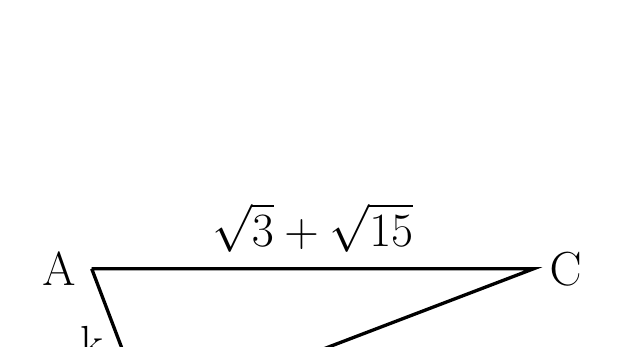
\begin{tikzpicture}
                \draw[very thick, black] (0,0) node[anchor=east]{A} -- node[anchor=east]{k}
                (0.71, -1.87) node[anchor=north]{B} -- node[anchor= north west]{$3+\sqrt{5}$}
                (5.61, 0) node[anchor=west]{C} -- node[anchor=south]{$\sqrt{3}+\sqrt{15}$}
                (0, 0);
                \coordinate (A) at (0, 0) {};
                \coordinate (B) at (0.71, -1.87) {};
                \coordinate (C) at (5.61, 0) {};
                \tkzMarkRightAngle[very thick, draw=black,size=.3](A,B,C);
            \end{tikzpicture}
            
            $ABC$ is a right angled triangle. $k$ is a positive integer.\\
            Find the value of $k$.
            \vspace{\stretch{2}}
        \end{subparts}
    \end{parts}
    \newpage

    % Question 2
    \question The Force, $F$, between two magnets is inversely proportional to the\\ square of the distance, $x$, between them.\\
    When $x=3$, $F=4$.
    \begin{parts}
        \part Find an expression for $F$ in terms of $x$.
        \vspace{\stretch{1}}
        \part Calculate $F$ when $x=2$.
        \vspace{\stretch{1}}
        \part Calculate $x$ when $F=64$.
        \vspace{\stretch{1}}
    \end{parts}
    \newpage

    % Question 3
    \question \phantom{1pt}\\
    \begin{minipage}{0.4\textwidth}
        \begin{tikzpicture}
            \coordinate (A) at (0, 0) {};
            \coordinate (B) at (0, 3) {};
            \coordinate (C) at (5, 0) {};
            \draw[very thick, black] (A)--(B)--node[anchor= south west]{$L$m}(C)--(A);
            \pic [very thick, draw, -, "$x\degree$", angle eccentricity=1.5, angle radius=1cm] {angle = B--C--A};
            \tkzMarkRightAngle[very thick, draw=black,size=.3](B,A,C);
        \end{tikzpicture}
    \end{minipage}
    \begin{minipage}{0.5\textwidth}
        You may use a calculator.\\ Elliott did an experiment to find the value of $g$ m/s$^2$, the acceleration due to gravity.
        He measured the time, $T$ s, that a block took to slide $L$ m down a smooth slope of angle $x\degree$.
    \end{minipage}
    
    \vspace{1cm}
    He then used the formula $g=\frac{2L}{T^2\sin(x\degree)}$ to calculate an estimate for $g$.

    $T=1.3$ correct to 1 decimal place. $L=4.50$ correct to 2 decimal places. $x=30$ correct to the nearest integer.

    \begin{parts}
        \part \label{part 1} Calculate the lower bound and the upper bound for the value of $g$.\\
        Give your answers correct to 3 decimal places.
        \vspace{\stretch{1}}\\
        \part Use your answer to part (\ref{part 1}) to write down the value of $g$ to a suitable degree of accuracy.\\ Explain your reasoning.
        \vspace{\stretch{1}}
    \end{parts}
    \newpage

    % Question 4
    \question Solve the simultaneous equations
    \begin{equation*}
        \begin{split}
            x^2+y^2&=29 \\
            y-x&=3
        \end{split}
    \end{equation*}
    \newpage

    % Question 5
    \question $$P=\frac{n^2+a}{n+a}$$
    Rearrange the formula to make $a$ the subject.
    \newpage

    % Question 6
    \question Simplify $$\frac{4x^2-9}{2x^2-5x+3}$$
    \newpage

    % Question 7
    \question Solve the equation $$\frac{7}{x+2} + \frac{1}{x-1}=4$$
    \newpage

    % Question 8
    \question The diagram shows a circle of radius 5cm, centred at the origin.\\
    \begin{center}
        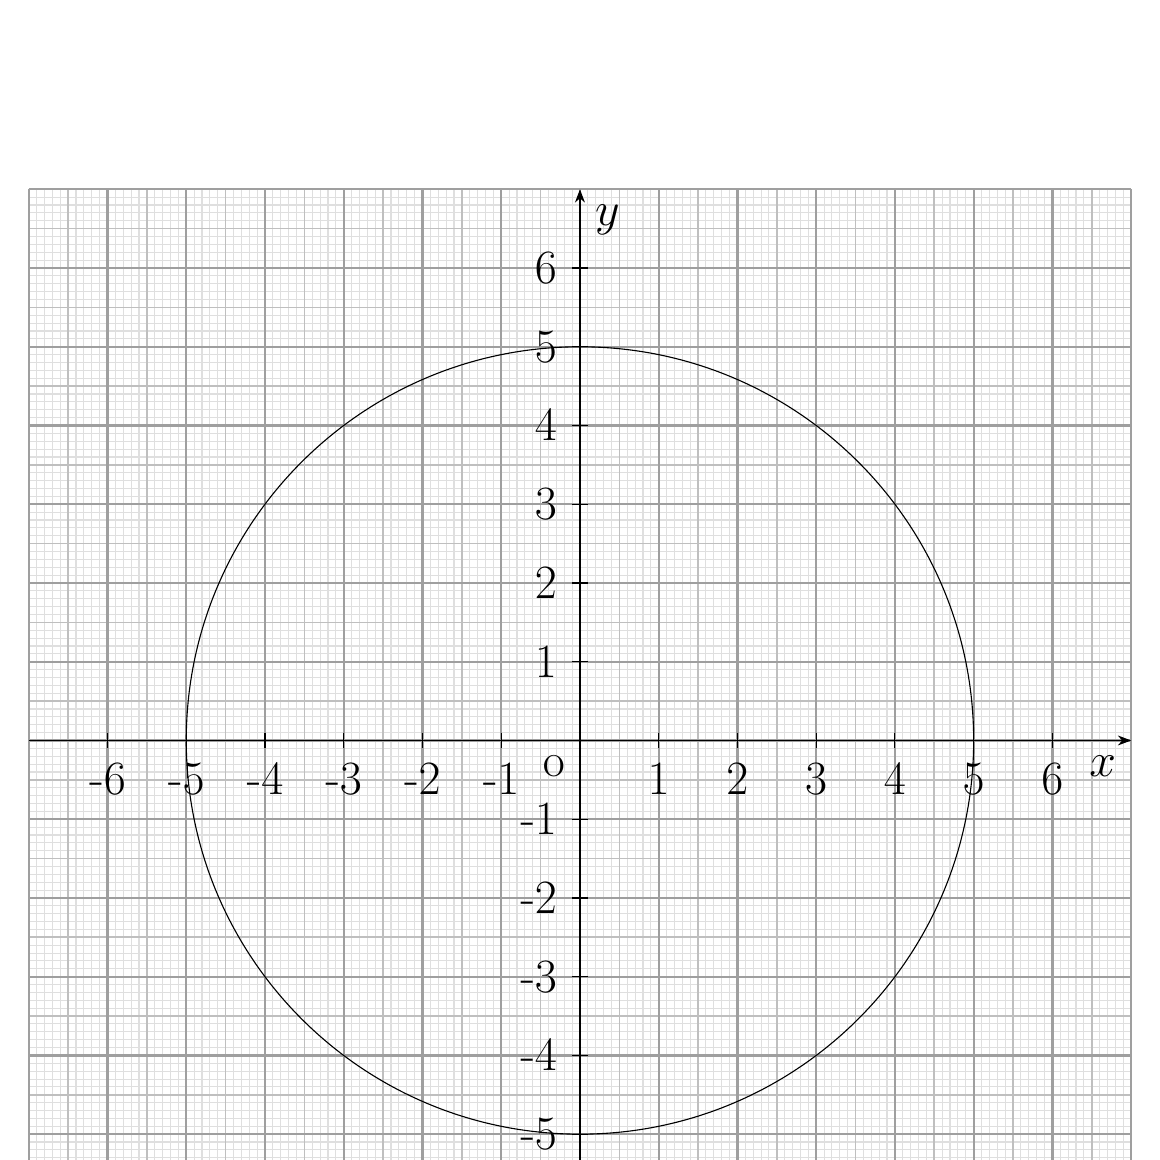
\begin{tikzpicture}
            % grid
            \draw[     thin,gray!25]   (-7,-7) grid[step= 1mm] ++ (14,14);
            \draw[semithick,gray!50]   (-7,-7) grid[step= 5mm] ++ (14,14);
            \draw[    thick,gray!75]   (-7,-7) grid[step=10mm] ++ (14,14);
            % axis
            \draw[-Stealth] (0,-7) -- (0,7) node[below right] {$y$};
            \draw[-Stealth] (-7,0) -- (7, 0) node[below  left] {$x$};
            \foreach \i in {-6,...,-1}{\draw (\i,1mm) -- + (0,-2mm) node[below] {\i};}
            \foreach \i in {1,...,6}{\draw (\i,1mm) -- + (0,-2mm) node[below] {\i};}
            \foreach \i in {-6,...,-1}{\draw (1mm,\i) -- + (-2mm,0) node[ left] {\i};}
            \foreach \i in {1,...,6}{\draw (1mm,\i) -- + (-2mm,0) node[ left] {\i};}
            % curve
            \draw (0,0) circle (5cm) node[anchor=north east]{o};
        \end{tikzpicture}
    \end{center}
    Draw a suitable straight line on the diagram to find estimates of the solutions to the pair of equations $$x^2+y^2=25 \text{ and } y=2x+1$$
    \newpage

    % Question 9
    \question A sketch of the curve $y=\sin{x\degree}$ for $0\leq x\leq 360$ is shown below.\\
    \vspace{5pt}
    \begin{tikzpicture}[scale=1.5]
        \begin{axis}[
            minor tick num=1,
            axis lines=center,
            extra y ticks= {0},
            xlabel=$x$,ylabel=$y$,
            xtick={0,90,...,360},
            ymax=2,
            ymin=-2,
            transform shape,
            ]
            \addplot[very thick, domain=0:360,samples=100]
            {sin(x)};
        \end{axis}
    \end{tikzpicture}\\
    Using the sketch above, or otherwise, find the equations of the following curves.\\
    
    \begin{minipage}{0.4\textwidth}
        \begin{tikzpicture}[scale=0.8]
            \begin{axis}[
                minor tick num=1,
                axis lines=center,
                extra y ticks= {0},
                xlabel=$x$,ylabel=$y$,
                xtick={0,90,...,360},
                ymax=2,
                ymin=-2,
                ]
                \addplot[very thick, domain=0:360,samples=100]
                {2*sin(x)};
            \end{axis}
        \end{tikzpicture}
    \end{minipage}
    \begin{minipage}{.2\textwidth}
        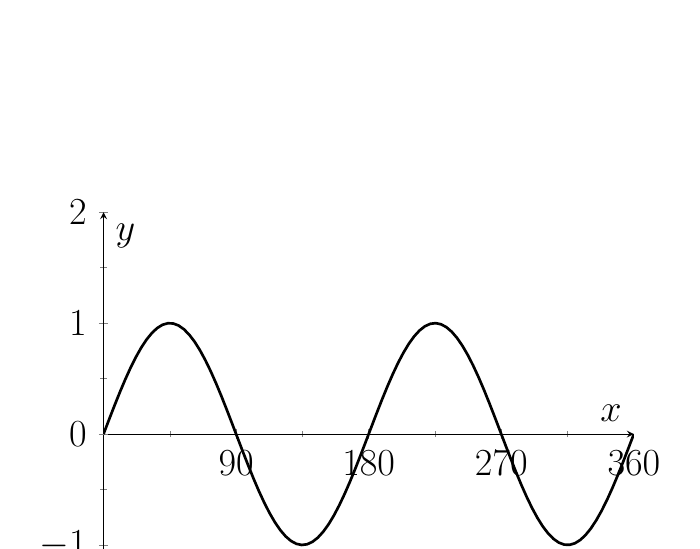
\begin{tikzpicture}[scale=0.8]
            \begin{axis}[
                minor tick num=1,
                axis lines=center,
                extra y ticks= {0},
                xlabel=$x$,ylabel=$y$,
                xtick={0,90,...,360},
                ymax=2,
                ymin=-2,
                ]
                \addplot[very thick, domain=0:360,samples=100]
                {sin(2*x)};
            \end{axis}
        \end{tikzpicture}
    \end{minipage}
    \newpage

    % Question 10
    \question The graph of $y=f(x)$ is shown on the grids.\\
    \begin{parts}
        \part On this grid, sketch the graph of $y=f(x)+1$\\
        \begin{center}
            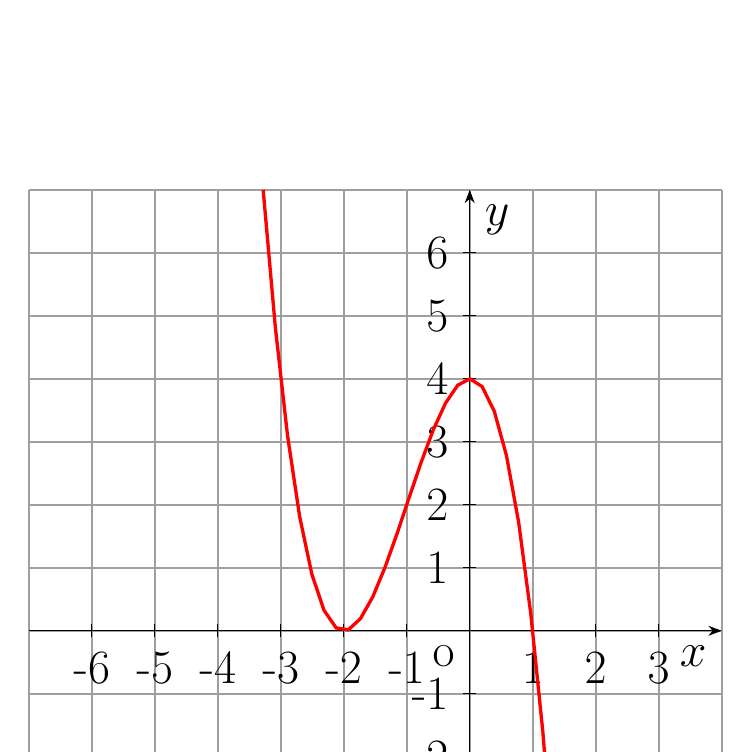
\begin{tikzpicture}[scale=0.8]
                % grid
                \draw[    thick,gray!75]   (-7,-4) grid[step=10mm] ++ (11,11);
                % axis
                \draw[-Stealth] (-7,0) -- (4, 0) node[below  left] {$x$};
                \draw[-Stealth] (0,-4) -- (0,7) node[below right] {$y$};
                \foreach \i in {-6,...,-1}{\draw (\i,1mm) -- + (0,-2mm) node[below] {\i};}
                \foreach \i in {1,...,3}{\draw (\i,1mm) -- + (0,-2mm) node[below] {\i};}
                \foreach \i in {-3,...,-1}{\draw (1mm,\i) -- + (-2mm,0) node[ left] {\i};}
                \foreach \i in {1,...,6}{\draw (1mm,\i) -- + (-2mm,0) node[ left] {\i};}
                % curve
                \draw[very thick, red]  plot[domain= -3.279:1.355] (\x, 4-3*\x*\x-\x*\x*\x);
                \draw (0,0) node[anchor=north east]{o};
            \end{tikzpicture}
        \end{center}
        \part On this grid, sketch the graph of $y=f(\frac{x}{2})$\\
        \begin{center}
            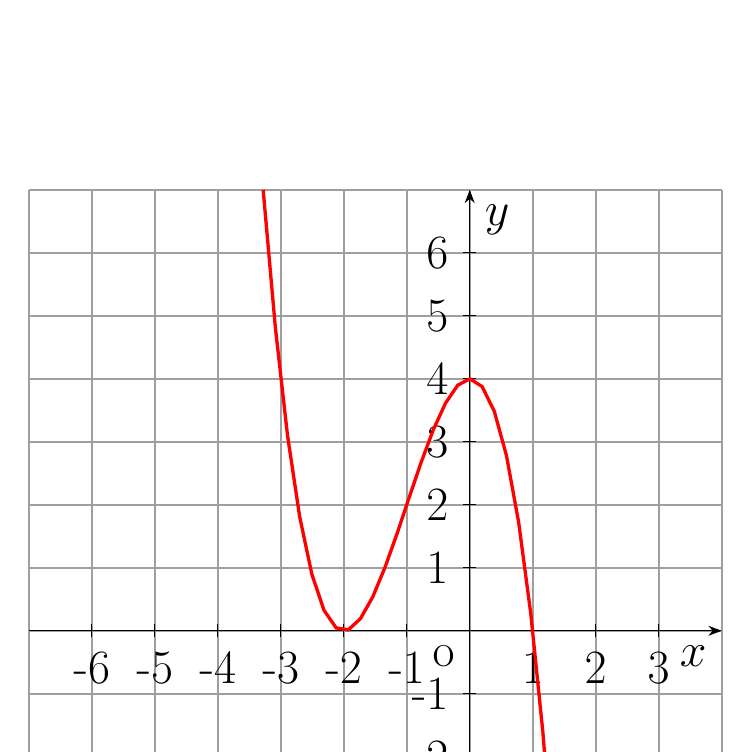
\begin{tikzpicture}[scale=0.8]
                % grid
                \draw[    thick,gray!75]   (-7,-4) grid[step=10mm] ++ (11,11);
                % axis
                \draw[-Stealth] (0,-4) -- (0,7) node[below right] {$y$};
                \draw[-Stealth] (-7,0) -- (4, 0) node[below  left] {$x$};
                \foreach \i in {-6,...,-1}{\draw (\i,1mm) -- + (0,-2mm) node[below] {\i};}
                \foreach \i in {1,...,3}{\draw (\i,1mm) -- + (0,-2mm) node[below] {\i};}
                \foreach \i in {-3,...,-1}{\draw (1mm,\i) -- + (-2mm,0) node[ left] {\i};}
                \foreach \i in {1,...,6}{\draw (1mm,\i) -- + (-2mm,0) node[ left] {\i};}
                % curve
                \draw[very thick, red]  plot[domain= -3.279:1.355] (\x, 4-3*\x*\x-\x*\x*\x);
                \draw (0,0) node[anchor=north east]{o};
            \end{tikzpicture}
        \end{center}
    \end{parts}
    \newpage

    % Question 11
    \question
    \begin{parts}
        \part Show that $$(2a-1)^2-(2b-1)^2=4(a-b)(a+b-1)$$\\
        \vspace{\stretch{1}}
        \part Prove that the difference between the squares of any two odd numbers is a multiple of 8.\\
        (Hint: an odd number is a multiple of 2 minus 1)\\
        \vspace{\stretch{1}}
    \end{parts}
    \newpage

    % Question 12
    \question The diagram below shows an irregular hexagon.\\
    All the corners are right angles.\\
    \begin{tikzpicture}[scale=0.6]
        \coordinate (A) at (0, 0) {};
        \coordinate (B) at (0, 6) {};
        \coordinate (C) at (2.5, 6) {};
        \coordinate (D) at (2.5,2.5) {};
        \coordinate (E) at (4.5, 2.5) {};
        \coordinate (F) at (4.5, 0) {};
        \draw[very thick, black]   (A)-- node[anchor= east]{$(2x+5)$}
                (B)-- node[anchor= south]{$(3x-2)$}
                (C)--
                (D)-- node[anchor= south]{$2$}
                (E)-- node[anchor= west]{$(3x-2)$}
                (F)--
                (A);
    \end{tikzpicture}\\
    The area of the shape is 25.\\
    Show that $6x^2+17x-39=0$
    \newpage

    % Question 13
    \question The expression $8x-x^2$ can be written in the form $p-(x-q)^2$,\\ for all values of $x$.
    \begin{parts}
        \part Find the value of $p$ and the value of $q$.\\
        \vspace{\stretch{2}}
        \part The expression $8x-x^2$ has a maximum value.\\
        \begin{subparts}
            \subpart Find the maximum value of $8x-x^2$.\\
            \vspace{\stretch{1}}
            \subpart State the value of $x$ for which this maximum value occurs.\\
            \vspace{\stretch{1}}
        \end{subparts}
    \end{parts}
    \newpage

    % Question 14
    \question You may use a calculator.\\The diagram represents a cuboid $ABCDEFGH$\\
    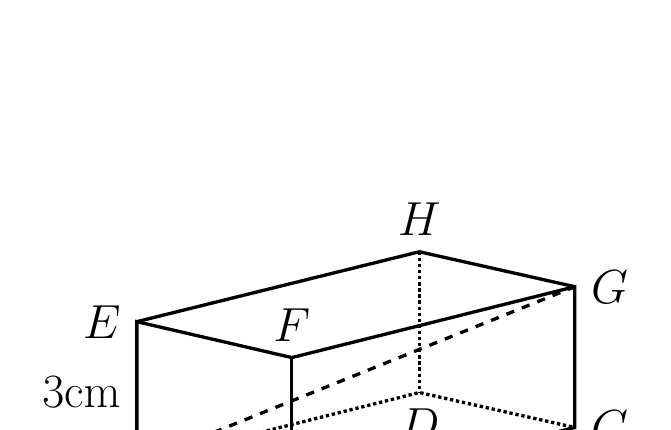
\begin{tikzpicture}[scale=0.6]
        \coordinate (A) at (0, 0) {};
        \coordinate (B) at (3.28,-0.74) {};
        \coordinate (C) at (9.27,0.76) {};
        \coordinate (D) at (5.98,1.5) {};
        \coordinate (E) at (0,3) {};
        \coordinate (F) at (3.28,2.24) {};
        \coordinate (G) at (9.27,3.74) {};
        \coordinate (H) at (5.98,4.48) {};
        \draw[very thick, black]   (A)node[anchor= east]{$A$}-- node[anchor= north]{5cm}
                (B)node[anchor= north]{$B$}-- node[anchor= north]{7cm}
                (C)node[anchor= west]{$C$}--
                (G)node[anchor= west]{$G$}--
                (F)node[anchor= south]{$F$}--
                (E)node[anchor= east]{$E$}-- node[anchor= east]{3cm}
                (A);
        \draw[very thick, black] (F)--(B);
        \draw[very thick, black] (G)--(C);
        \draw[very thick, black] (G)--(H)--(E);
        \draw[densely dotted, very thick] (H)node[anchor= south]{$H$}--(D)node[anchor= north]{$D$};
        \draw[densely dotted, very thick] (A)--(D)--(C);
        \draw[dashed, very thick] (A)--(G);
    \end{tikzpicture}\\
    $AB=5$cm. $BC=7$cm. $AE=3$cm.\\
    \begin{parts}
        \part Calculate the length of $AG$.\\
        Give your answer correct to 3 significant figures.\\
        \vspace{\stretch{1}}
        \part Calculate the size of the angle between $AG$ and the face $ABCD$.\\
        Give your answer correct to 1 decimal place.
        \vspace{\stretch{1}}
    \end{parts}
    \newpage

    % Question 15
    \question The shape is a model of a concrete post. It is a cuboid with a pyramid on top.\\
    
    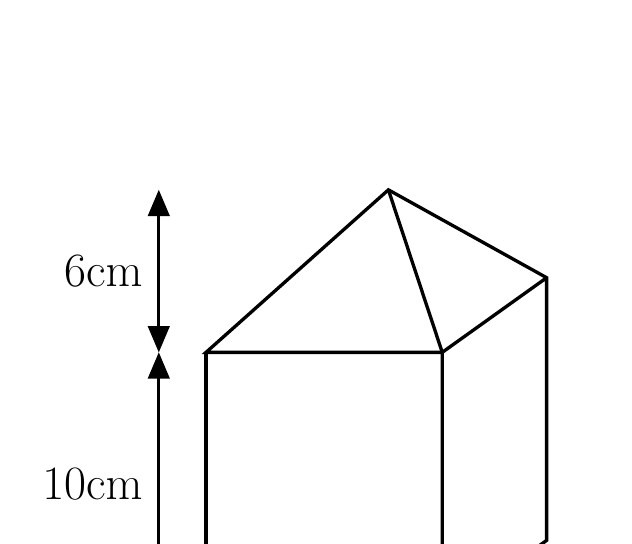
\begin{tikzpicture}[scale=0.6]
        \coordinate (X) at (-1, 0) {};
        \coordinate (Y) at (-1, 5.56) {};
        \coordinate (Z) at (-1, 9) {};
        \coordinate (A) at (0, 0) {};
        \coordinate (B) at (5,0) {};
        \coordinate (C) at (7.21,1.58) {};
        \coordinate (D) at (7.21,7.14) {};
        \coordinate (E) at (5,5.56) {};
        \coordinate (F) at (0,5.56) {};
        \coordinate (G) at (3.86,9) {};
        \draw[very thick, black]   (A)-- node[anchor= north]{5cm}
                (B)-- node[anchor= north west]{5cm}
                (C)--
                (D)--
                (G)--
                (F)-- 
                (E)--
                (D);
        \draw[very thick, black] (B)--(E)--(G);
        \draw[very thick, black] (A)--(F);
        \draw[very thick, black, triangle 45-triangle 45] (X) -- node[anchor= east]{10cm} (Y);
        \draw[very thick, black, triangle 45-triangle 45] (Y) -- node[anchor= east]{6cm} (Z);
    \end{tikzpicture}\\
    
    \begin{parts}
        \part Calculate the volume of the model.
        \vspace{\stretch{1}}\\
        \part The model is built to a scale of 1:30 and the surface area is 290cm$^2$.\\
        Calculate the surface area of the actual post.\\
        Give your answer in square metres.
        \vspace{\stretch{1}}
    \end{parts}
    \newpage

    % Question 16
    \question \phantom{1pt}\\
    \begin{tikzpicture}[scale=0.6]
        \coordinate (P) at (11.5, 19.52) {};
        \coordinate (S) at (5.95,10.03) {};
        \coordinate (T) at (17.1,10.03) {};
        \coordinate (O) at (11.5,6.48) {};
        \coordinate (Q) at (0,0) {};
        \coordinate (R) at (23,0) {};
        \draw[very thick, black]   (S)node[anchor= east]{$S$}--
                (R)node[anchor= north]{$R$}--
                (P)node[anchor= south]{$P$}--
                (Q)node[anchor= north]{$Q$}--
                (T)node[anchor= west]{$T$};
        \draw (O)node[anchor=north]{$O$};
        \draw[very thick, black] (O) circle (6.62);
    \end{tikzpicture}\\
    $S$ and $T$ are points on a circle, centre $O$.\\
    $PSQ$ and $PTR$ are tangents to the circle.\\
    $SOR$ and $TOQ$ are straight lines.\\

    Prove that triangle $PQT$ and triangle $PRS$ are congruent.
    \newpage

    % Question 17
    \question \phantom{1pt}\\
    \begin{tikzpicture}[scale=0.6]
        \coordinate (O) at (0,0) {};
        \coordinate (A) at (6.95,9.95) {};
        \coordinate (B) at (24.88,9.95) {};
        \coordinate (C) at (18,0) {};
        \coordinate (P) at (14.27,3.37) {};
        \draw[very thick, black]   (A)node[anchor= south]{$A$}--
                (B)node[anchor= south]{$B$}--
                (C)node[anchor= north]{$C$};
        \draw[very thick, black] (O) -- (A);
        \draw[very thick, black] (O) -- (C);
        \draw[very thick, black] (O)node[anchor= north]{$O$} -- (P)node[anchor= south west]{$P$};
        \draw[very thick, black] (A) -- (C);
    \end{tikzpicture}\\
    $OABC$ is a parallelogram.\\
    $P$ is the point on $AC$ such that $AP=\frac{2}{3}AC$.\\
    $\overrightarrow{OA}=6\textbf{a}$. $\overrightarrow{OC}=6\textbf{c}$.
    \begin{parts}
        \part Find the vector $\overrightarrow{OP}$.\\
        Give your answer in terms of $\textbf{a}$ and $\textbf{c}$.
        \vspace{\stretch{1}}\\
        The midpoint of $CB$ is $M$.
        \part Prove that $OPM$ is a straight line.
        \vspace{\stretch{1}}
    \end{parts}
    \newpage

    % Question 18
    \question \phantom{1pt}\\
     \begin{tikzpicture}[scale=0.8]
        \coordinate (A) at (7.99,3.25) {};
        \coordinate (B) at (0,0) {};
        \coordinate (C) at (9.91,-1.24) {};
        \coordinate (D) at (2.44,0.98) {};
        \draw[very thick, black]   (A)node[anchor= south]{$A$}--
                (B)node[anchor= north]{$B$}--
                (C)node[anchor= north]{$C$} -- (A);
        \tkzMarkRightAngle[very thick, draw=black,size=.6](B,A,C);
        \filldraw[color=black] (D) circle [radius=.1] node[anchor= south]{$D$};
    \end{tikzpicture}\\
    $ABC$ is a right angled triangle.\\
    $D$ is the point on $AB$ such that $AD=3DB$.\\
    Additionally $AC=2DB$.\\

    Show that $\sin{C}=\frac{k}{\sqrt{20}}$, where $k$ is an integer.\\

    Write down the value of $k$.
    \newpage

    % Question 19
    \question \phantom{1pt}\\
    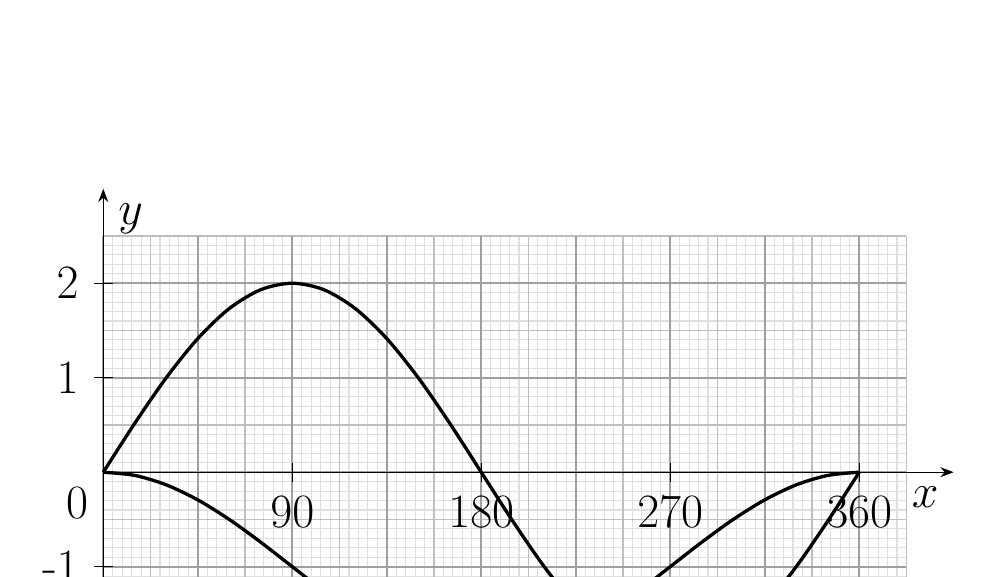
\begin{tikzpicture}[scale=1.2]
        % grid
        \draw[thin,gray!25] (0,-2.5) grid[step=1mm] (8.5,2.5);
        \draw[semithick,gray!50] (0,-2.5) grid[step=5mm] (8.5,2.5);
        \draw[thick,gray!75] (0,-2.5) grid[step=10mm] (8.5,2.5);
    
        % axis
        \draw[-Stealth] (0,-2.5) -- (0,3) node[below right] {$y$};
        \draw[-Stealth] (0,0) -- (9,0) node[below left] {$x$};
    
        % x-axis labels
        \foreach \i in {90,180,270,360}
            \draw (\i/45,1mm) -- + (0,-2mm) node[below] {\i};
   
        % y-axis labels
        \foreach \i in {-2,-1,1,2}
            \draw (1mm,\i) -- + (-2mm,0) node[left] {\i};
   
        % plot 2*sin(x)
        \draw[domain=0:8,smooth,variable=\x,black,very thick] plot ({\x},{2*sin((\x r)*(pi/4))});
   
        % plot cos(x) - 1
        \draw[domain=0:8,smooth,variable=\x,black,very thick] plot ({\x},{cos((\x r)*(pi/4)) - 1});
   
        % label the origin
        \node[anchor=north east] at (0,0) {0};
    \end{tikzpicture}\\
    The diagram shows part of 2 graphs.\\
    The equation of one graph is $y=a\sin(x\degree)$\\
    The equation of the other graph is $y=\cos(x\degree)+b$\\
    \begin{parts}
        \part Use the graphs to find the value of $a$ and the value of $b$.\\
        \vspace{\stretch{1}}\\
        \part Use the graphs to find the values of $x$ in the range $0\degree\leq x\leq 720\degree$ when $a\sin(x\degree)=\cos(x\degree)+b$.\\
        \vspace{\stretch{1}}\\
        \part Use the graphs to find the value of $a\sin(x\degree)-(\cos(x\degree)+b)$ when $x=450\degree$.\\
        \vspace{\stretch{1}}\\
    \end{parts}
    \newpage

    % Question 20
    \question \phantom{1pt}
    \begin{center}
        \begin{tikzpicture}[scale=0.6]
            \coordinate (A) at (12.26,7.52) {};
            \coordinate (B) at (0,0) {};
            \coordinate (C) at (15,0) {};
            \draw[very thick, black] (A)node[anchor= south]{$A$}--
                    (B)node[anchor= north]{$B$}-- node[anchor= north]{$15cm$}
                    (C)node[anchor= north]{$C$}-- node[anchor= south west]{$8cm$}(A);
            \pic [very thick, draw, -, "$70\degree$", angle eccentricity=1.5, angle radius=1cm] {angle = A--C--B}; 
        \end{tikzpicture}
    \end{center}
    You may use a calculator.\\
    \begin{parts}
        \part Calculate the length of $AB$.\\
        Give your answer correct to 3 significant figures.\\
        \vspace{\stretch{1}}\\
        \part Calculate the size of angle $BAC$.\\
        Give your answer correct to 1 decimal place.\\
        \vspace{\stretch{1}}\\
    \end{parts}
    \newpage

    % Question 21
    \question The radius of a sphere is 3cm.\\
    The radius of the base of a cone is also 3cm.\\
    The volume of the sphere is 3 times the volume of the cone.\\

    Work out the curved surface area of the cone.\\
    Give your answer as a multiple of $\pi$.
    \newpage

    % Question 22
    \question You may use a calculator.
    \begin{center}
        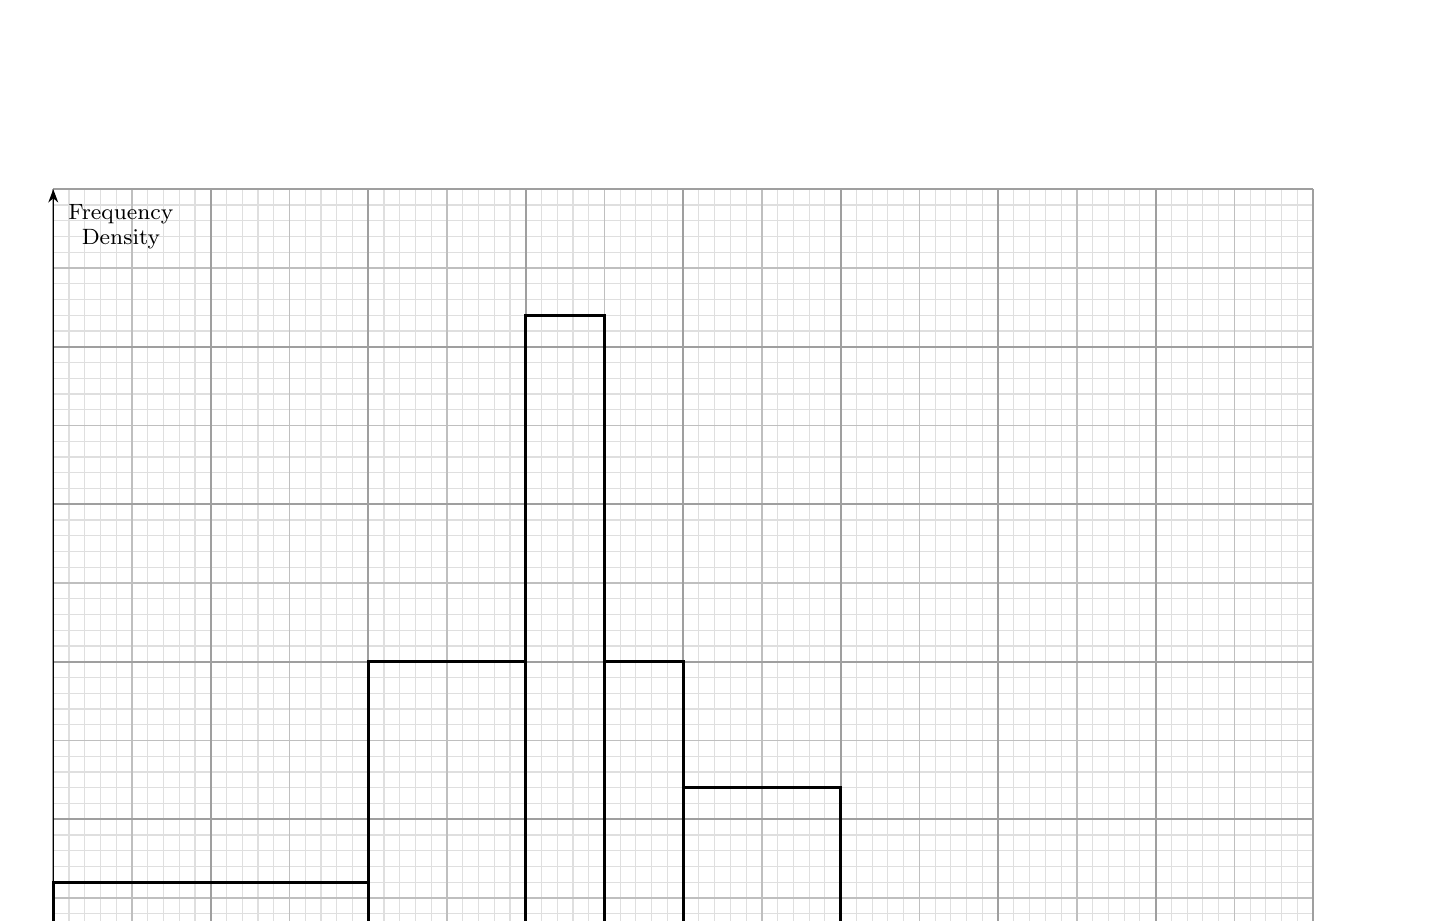
\begin{tikzpicture}[scale=2]  % Set font size to small for labels
            % grid
            \draw[thin,gray!25] (0,0) grid[step=1mm] (8,5);
            \draw[semithick,gray!50] (0,0) grid[step=5mm] (8,5);
            \draw[thick,gray!75] (0,0) grid[step=10mm] (8,5);
        
            % axis
            \draw[-Stealth] (0,0) -- (0,5) node[below right, align=center, font=\tiny] {Frequency\\Density};
            \draw[-Stealth] (0,0) -- (8,0) node[right, align=center, font=\tiny] {Time in\\Seconds};

            % x-axis labels
            \foreach \i in {5,10,...,35,40}
                \draw (\i/5,1mm) -- + (0,-2mm) node[below] {\i};
                 % x-axis labels (Time in Seconds)

            % label the origin
            \draw (0,1mm) -- + (0,-2mm) node[below] {0};
        
            % histogram bars
            \draw[very thick] (0,0) rectangle (2,0.6);
            \draw[very thick] (2,0) rectangle (3,2);
            \draw[very thick] (3,0) rectangle (3.5,4.2);
            \draw[very thick] (3.5,0) rectangle (4,2);
            \draw[very thick] (4,0) rectangle (5,1.2);
            \draw[very thick] (5,0) rectangle (8,0.2);
        
        \end{tikzpicture}
    \end{center}
    The histogram shows information about the time it took some children to connect to the internet.\\
    None of the children took more than 40 seconds to connect to the internet.\\

    110 children took up to 12.5 seconds to connect to the internet.\\
    Work out the number of children who took 21 seconds or more to connect to the internet.
    \newpage

    % Question 23
    \question Stefan's drawer contains 5 white socks and 3 black socks.\\
    He takes out two socks at random.\\

    Work out the probability that Stefan takes out two socks of the same colour.
\end{questions}

\newpage
\begin{titlepage}
    \begin{center}

        \vspace*{\fill}
        \Huge \textbf{Part 2: The Test}\\
        \vspace*{1cm}
        \vspace*{1cm}
        \large \textbf{The woes begin}\\
        \vspace*{\fill}
        
    \end{center}
\end{titlepage}
\newpage
%%%%%%%%%%%%%%%%%%%%%%%%%%% Part 2

\begin{questions}
    
    % Question 1
    \question You may use a calculator. Island X is a small island.\\
    In the winter of 1986 the ratio of natives to tourists on the island was $7:1$.\\
    In the summer of 1987 the ratio of natives to tourists on the island was $155:69$.\\
    The number of natives on the island decreased by 100 from the winter of 1986 to summer of 1987.\\
    The number of tourists on the island increased by 220 from the winter of 1986 to summer of 1987.\\

    Find the number of tourists that were there on Island X in the winter of 1986.
    \newpage

    % Question 2
    \question You may use a calculator. Find $P(B\cap\Bar{A}\ | C )$.\\
    Give your answer as a fraction in the form $\frac{a}{b}$ where $a$ and $b$ are integers.
    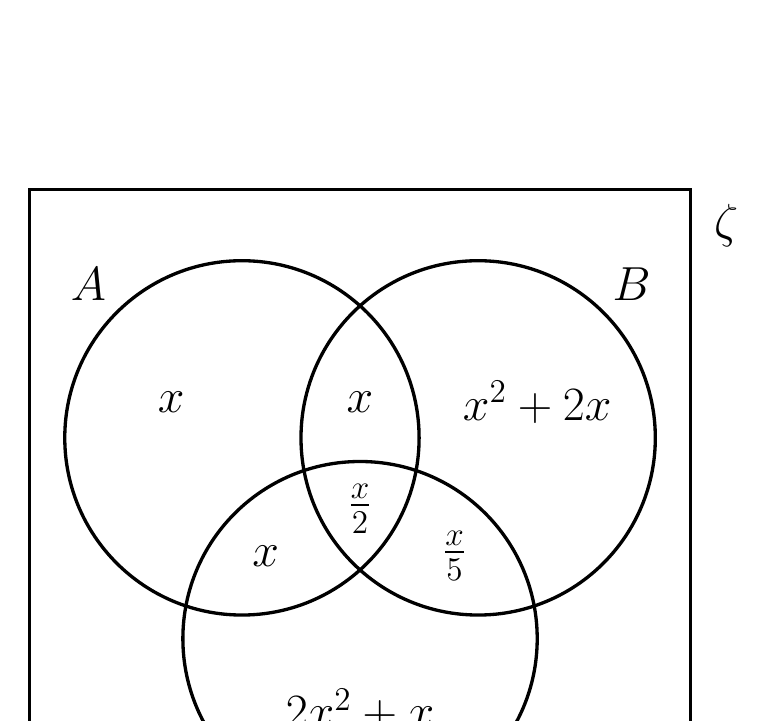
\begin{tikzpicture}[scale=1.5]
    
        % Define the three circles
        \begin{scope}
            \draw[very thick] (1.8,3.5) circle (1.5cm);
            \draw[very thick] (3.8,3.5) circle (1.5cm);
            \draw[very thick] (2.8,1.8) circle (1.5cm);
        \end{scope}
        
        % Draw the rectangle around the circles
        \draw[very thick] (0,0) rectangle (5.6,5.6);
        \node at (5.9,5.3) {$\zeta$};
        
        % Label the regions
        \node at (1.2,3.8) {$x$};
        \node at (4.3,3.8) {$x^2+2x$};
        \node at (2.8,1.2) {$2x^2+x$};
        \node at (2.8,2.9) {$\frac{x}{2}$};
        \node at (3.6,2.5) {$\frac{x}{5}$};
        \node at (2,2.5) {$x$};
        \node at (2.8,3.8) {$x$};
        \node at (4.8,0.4) {$13x-1$};
        \node at (0.5,4.8) {$A$};
        \node at (5.1,4.8) {$B$};
        \node at (1.3,0.4) {$C$};
    
    \end{tikzpicture}
    \newpage

    % Question 3
    \question The diagram below shows part of the graph of $y=2f(x-1)$
    \begin{center}
        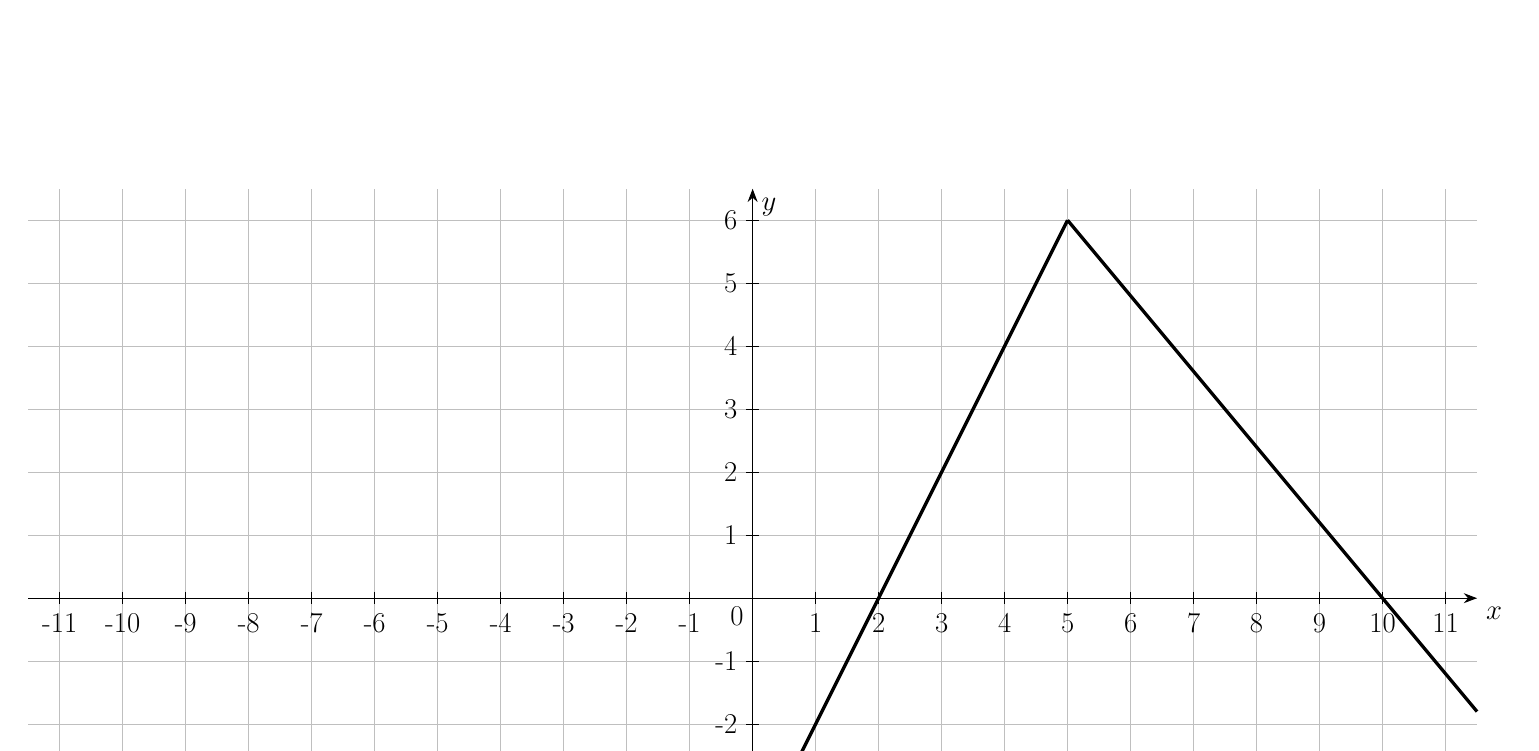
\begin{tikzpicture}[scale=0.8, every node/.style={scale=0.6}]
            % grid
            \draw[thin,gray!50] (-11.5,-4.5) grid[step=1] (11.5,6.5);
        
            % axis
            \draw[-Stealth] (0,-4.5) -- (0,6.5) node[below right] {$y$};
            \draw[-Stealth] (-11.5,0) -- (11.5,0) node[below right] {$x$};
        
            % x-axis labels
            \foreach \i in {-11,-10,...,-2,-1,1,2,...,11}
                \draw (\i,1mm) -- + (0,-2mm) node[below] {\i};
       
            % y-axis labels
            \foreach \i in {-4,-3,-2,-1,1,2,...,6}
                \draw (1mm,\i) -- + (-2mm,0) node[left] {\i};
       
            \draw[domain=-0.25:5,smooth,variable=\x,black,very thick] plot ({\x},{2*(\x)-4});
       
            \draw[domain=5:11.5,smooth,variable=\x,black,very thick] plot ({\x},{-1.2*(\x)+12});
       
            % label the origin
            \node[anchor=north east] at (0,0) {0};
        \end{tikzpicture}
    \end{center}
    
    On the grid below, draw the graph of $y=-f(-x)$
    \begin{center}
        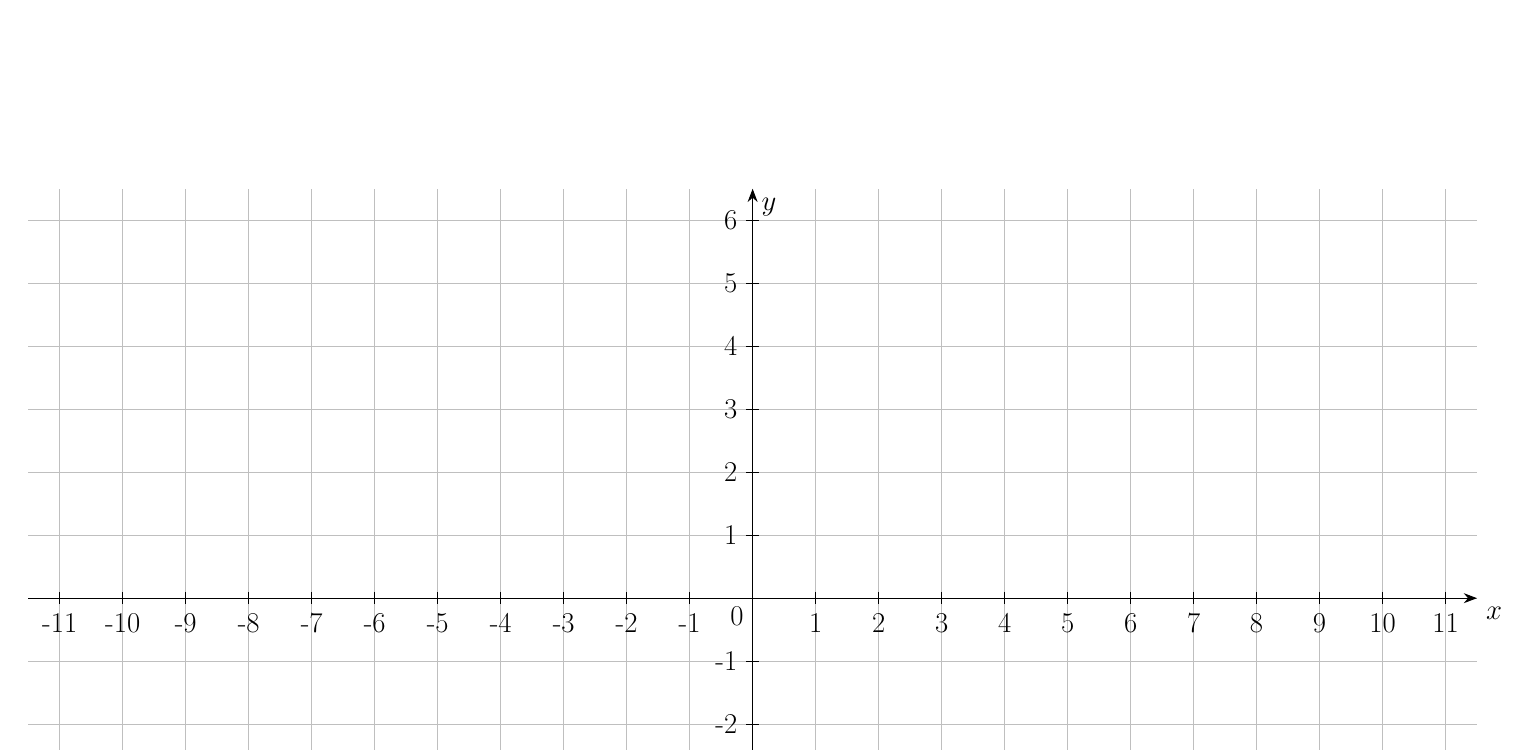
\begin{tikzpicture}[scale=0.8, every node/.style={scale=0.6}]
            % grid
            \draw[thin,gray!50] (-11.5,-4.5) grid[step=1] (11.5,6.5);
        
            % axis
            \draw[-Stealth] (0,-4.5) -- (0,6.5) node[below right] {$y$};
            \draw[-Stealth] (-11.5,0) -- (11.5,0) node[below right] {$x$};
        
            % x-axis labels
            \foreach \i in {-11,-10,...,-2,-1,1,2,...,11}
                \draw (\i,1mm) -- + (0,-2mm) node[below] {\i};
       
            % y-axis labels
            \foreach \i in {-4,-3,-2,-1,1,2,...,6}
                \draw (1mm,\i) -- + (-2mm,0) node[left] {\i};
       
            % label the origin
            \node[anchor=north east] at (0,0) {0};
        \end{tikzpicture}
    \end{center}
    \newpage

    % Question 4
    \question Using algebra, show that part of the line $3x+4y=0$ is a diameter of the circle with equation $x^2+y^2=25$.
    \newpage

    % Question 5
    \question Sue is making a toy rocket in her science lesson which is to be launched from the ground.\\
    The flight path of the toy rocket can be modelled by the equation\\ $h=-2t^2+6t+1$.\\
    $h$ is the height in metres the rocket reaches above the ground.\\
    $t$ is the time in seconds after the rocket is launched.\\

    Find the maximum height above the ground that the rocket reaches and the time it takes to reach this height.
    \newpage

    % Question 6
    \question Shape A is a regular polygon.\\
    The ratio of the size of the interior angle to the size of the exterior angle is $7:2$.
    The ratio of the side length to the number of sides is $5:3$.\\
    Find the perimeter of shape A.
    \newpage

    % Question 7
    \question You may use a calculator. Jamal is going to paddle between 3 points on a large lake.
    Jamal will start from Point A and paddle on a bearing of $050\degree$ until he reaches Point B. Once at Point B, Jamal will then paddle 1.6km on a bearing of $142\degree$ to reach Point C. Finally, Jamal will paddle directly to Point A from Point C where he will finish.
    The bearing of Point C from Point A is $098\degree$.\\

    Given that Jamal can paddle at an average speed of 7.2kph, find the time it will take him to paddle directly back to Point A from Point C. Give your answer to the nearest minute.
    \newpage

    % Question 8
    \question Triangle $ABC$ is an isosceles triangle.\\
    The points $X$ and $Y$ lie on the line $AC$.\\
    $AB=BC$.\\
    $AY=3AX$.\\
    $AC=4AX$.\\
    Prove that triangle $ABX$ and triangle $CBY$ are congruent.
    \newpage

    % Question 9
    \question Company T are designing a toy to be sold online.\\
    The toy will be made up of a hemisphere with radius $Xcm$ and a right cone with radius $Xcm$ and heigh $Ycm$.\\
    The cone will be attached to the top of the hemisphere.\\

    Given that the total mass of the toy is $100\pi$ grams and the density of the toy is $60g/cm^3$, express $Y$ in terms of $X$. Give your answer in the simplest form.
    \newpage

    % Question 10
    \question There are $N$ boys in a class at school.\\
    For every 2 boys in the class there are 3 girls in the class.\\
    3 students are chosen at random and taken out of the class.\\

    Given that the probability of choosing 3 boys is $\frac{1}{30}$, \\show that $23N^2-114N+88=0$
    \newpage

    % Question 11
    \question Consider 2 lines. Line A and Line B.\\
    Line A has gradient 2.\\
    Line B is perpendicular to Line A.\\
    Line A and Line B intersect at the Point $P(p,q)$.\\
    Line B crosses the $y$-axis at Point B.\\

    Show that the coordinates of Point B can be written as $(0,\frac{p}{2}+q)$.
    \newpage

    % Question 12
    \question The graphs of $y=2\cos{x}$ and $y=\sin{x}$ are shown in the diagram below for $0\leq x\leq 360\degree$.\\
    \begin{nscenter}
        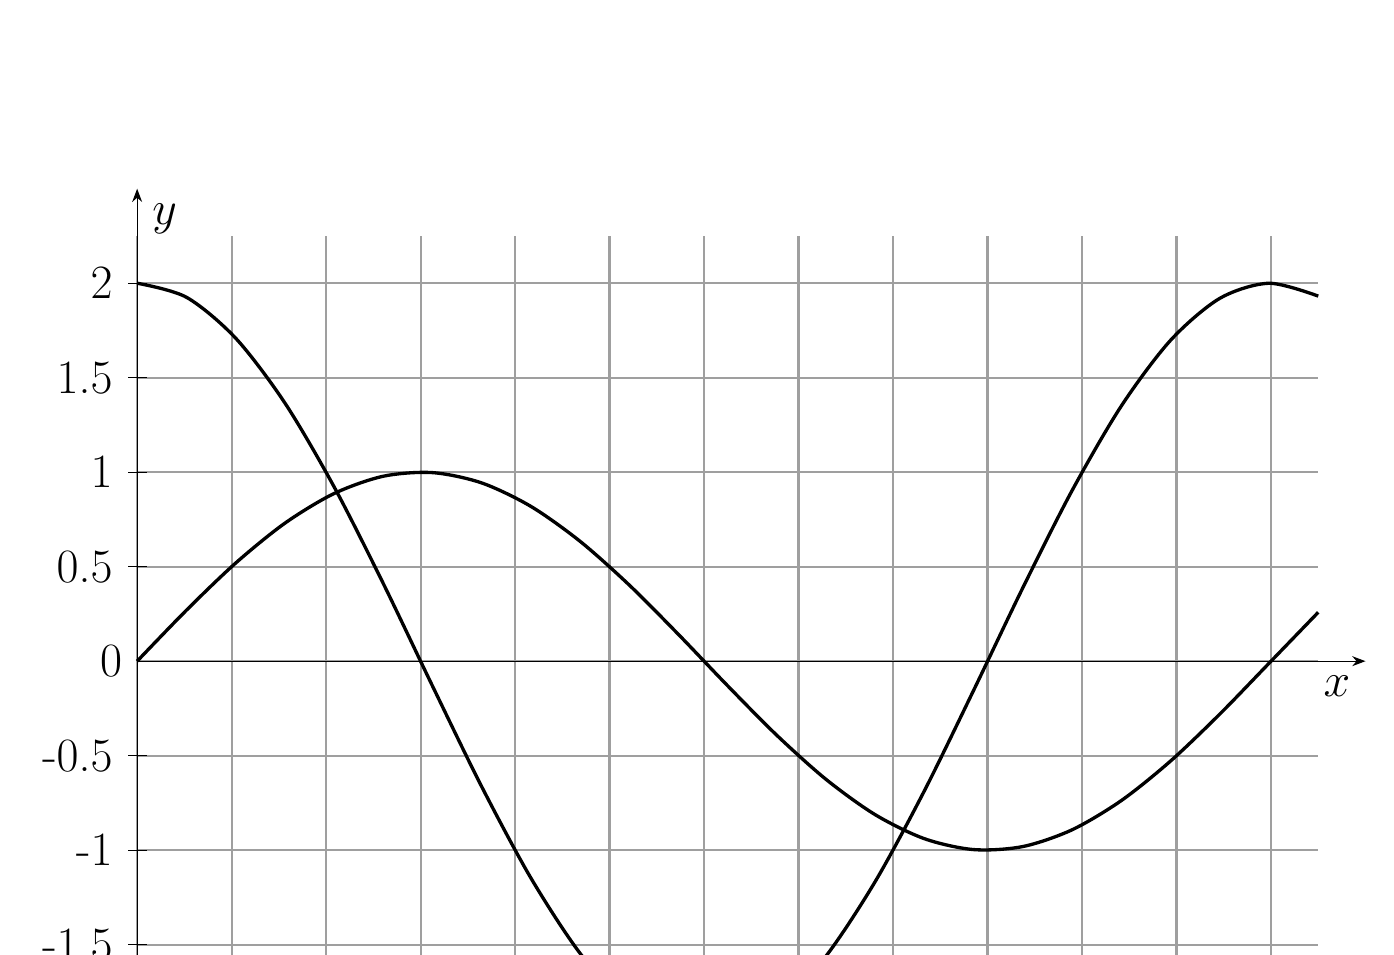
\begin{tikzpicture}[scale=1.2]
            % grid
            \draw[thick,gray!75] (0,-4.5) grid[step=10mm] (12.5,4.5);
    
            % axis
            \draw[-Stealth] (0,-4.5) -- (0,5) node[below right] {$y$};
            \draw[-Stealth] (0,0) -- (13,0) node[below left] {$x$};
    
            % y-axis labels
            \foreach \i in {-2,-1.5,-1,-0.5,0.5,1,1.5,2}
            \draw (1mm,2*\i) -- + (-2mm,0) node[left] {\i};
    
            % plot 2*sin(x)
            \draw[domain=0:12.5,smooth,variable=\x,black,very thick] plot ({\x},{4*cos((\x r)*(2 * pi)/12)});
    
            % plot cos(x) - 1
            \draw[domain=0:12.5,smooth,variable=\x,black,very thick] plot ({\x},{2*sin((\x r)*(2 * pi)/12))});
    
            % label the origin
            \node[anchor=east] at (0,0) {0};
        \end{tikzpicture}\\
    \end{nscenter}
    Use the graphs to find estimates for the solutions of the equation:\\
    \begin{equation*}
        \sin{x}-2\cos{x}=0 \text{ for } 0\leq x \leq 360\degree
    \end{equation*}        
    \newpage

    % Question 13
    \question The diagram below shows the graph of the equation $x^2+y^2=8$ and part of the graph of the equation $y=\frac{1}{x^2}+1$.\\
    \begin{nscenter}
        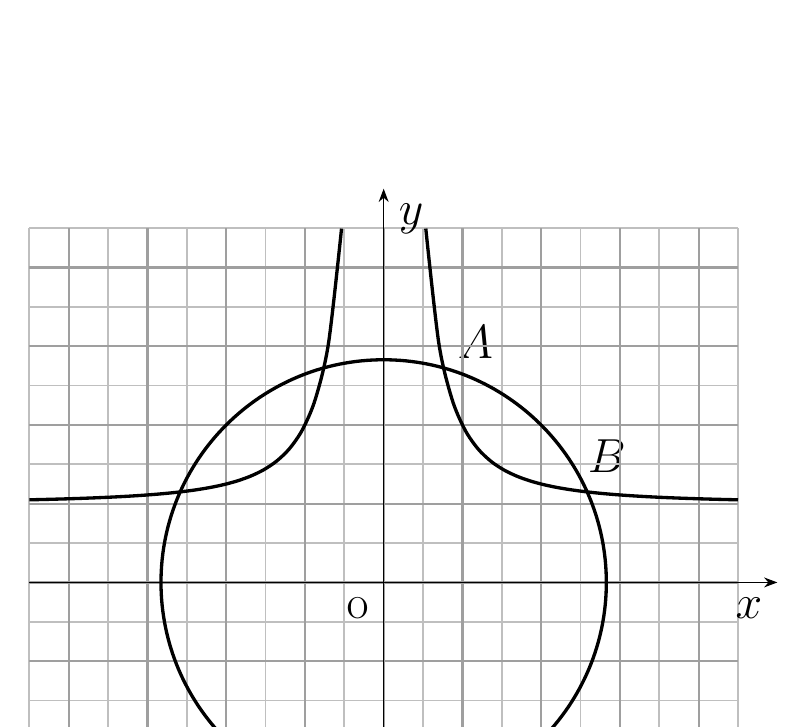
\begin{tikzpicture}[scale=1]
            % grid
            \draw (0.75,2.65)node[anchor=south west]{$A$};
            \draw (2.4,1.2)node[anchor=south west]{$B$};
            \draw[semithick,gray!50] (-4.5,-3.5) grid[step=5mm] (4.5,4.5);
            \draw[thick,gray!75] (-4.5,-3.5) grid[step=10mm] (4.5,4.5);
        
            % axis
            \draw[-Stealth] (0,-3.5) -- (0,5) node[below right] {$y$};
            \draw[-Stealth] (-4.5,0) -- (5,0) node[below left] {$x$};
       
            % plot 1
            \draw[domain=-4.5:-0.535,smooth,variable=\x,black,very thick] plot ({\x},{1/(\x * \x)+1});
            \draw[domain=0.535:4.5,smooth,variable=\x,black,very thick] plot ({\x},{1/(\x * \x)+1});
       
            % plot 2
            \draw[black,very thick] (0,0) circle (2.828);
       
            % label the origin
            \node[anchor=north east] at (0,0) {o};
        \end{tikzpicture}
    \end{nscenter}
    The points $A(p,q)$ and $B(r,s)$ are two of the points where\\ the graphs intersect.\\
    \begin{parts}
        \part Using the graphs above, find the solutions to the simultaneous equations:
        \begin{equation*}
            y=\frac{1}{x^2}+1
        \end{equation*}
        \begin{equation*}
            x^2+y^2=8\text{.}
        \end{equation*}
        Giving your answer in terms of $p$,$q$,$r$, and $s$.\\
        \vspace{\stretch{1}}\\
        There are 2 real solutions to the simultaneous equations: $x^2+y^2=8$ and $x=a$.
        \part Find the set of values of $a$ giving your answer in simplified surd form.
        \vspace{\stretch{1}}
    \end{parts}
    \newpage

    % Question 14
    \question The students in Class X and Class Y sat the same maths exam.\\
    Information is given about the performance of each class in the table below.
    \begin{nscenter}
        \begin{tabular}{|c|c|c|}
            \hline
            & X & Y\\
            \hline
            Lowest Score & $x-1$ \phantom{1pt} & $y+1$ \phantom{1pt}\\
            \hline
            Lower Quartile & $x+2$ \phantom{1pt} & $2(y+1)$ \phantom{1pt}\\
            \hline
            Median & $x^2-3$ \phantom{1pt} & $y(y-1)$ \phantom{1pt}\\
            \hline
            Upper Quartile & $4x+2$ \phantom{1pt} & $3y+1$ \phantom{1pt}\\
            \hline
            Highest Score & $2(x^2+2)$ \phantom{1pt} & $5y-4$ \phantom{1pt}\\
            \hline
        \end{tabular}
    \end{nscenter}\\
    The median score for Class X was half the median score for Class Y.\\
    The interquartile range for Class X was three times the interquartile range for Class Y.\\

    Michael scored 17 marks in his maths exam.\\
    Complete the following sentence;\\
    \begin{nscenter}
        \textit{"Michael was in the top \_\_\_ \% of performers in Class \_\_\_"}
    \end{nscenter}
    \newpage

    % Question 15
    \question The diagram below shows parts of the cubic graph of $y=f(x)$ and the linear graph of $y=g(x)$.\\
    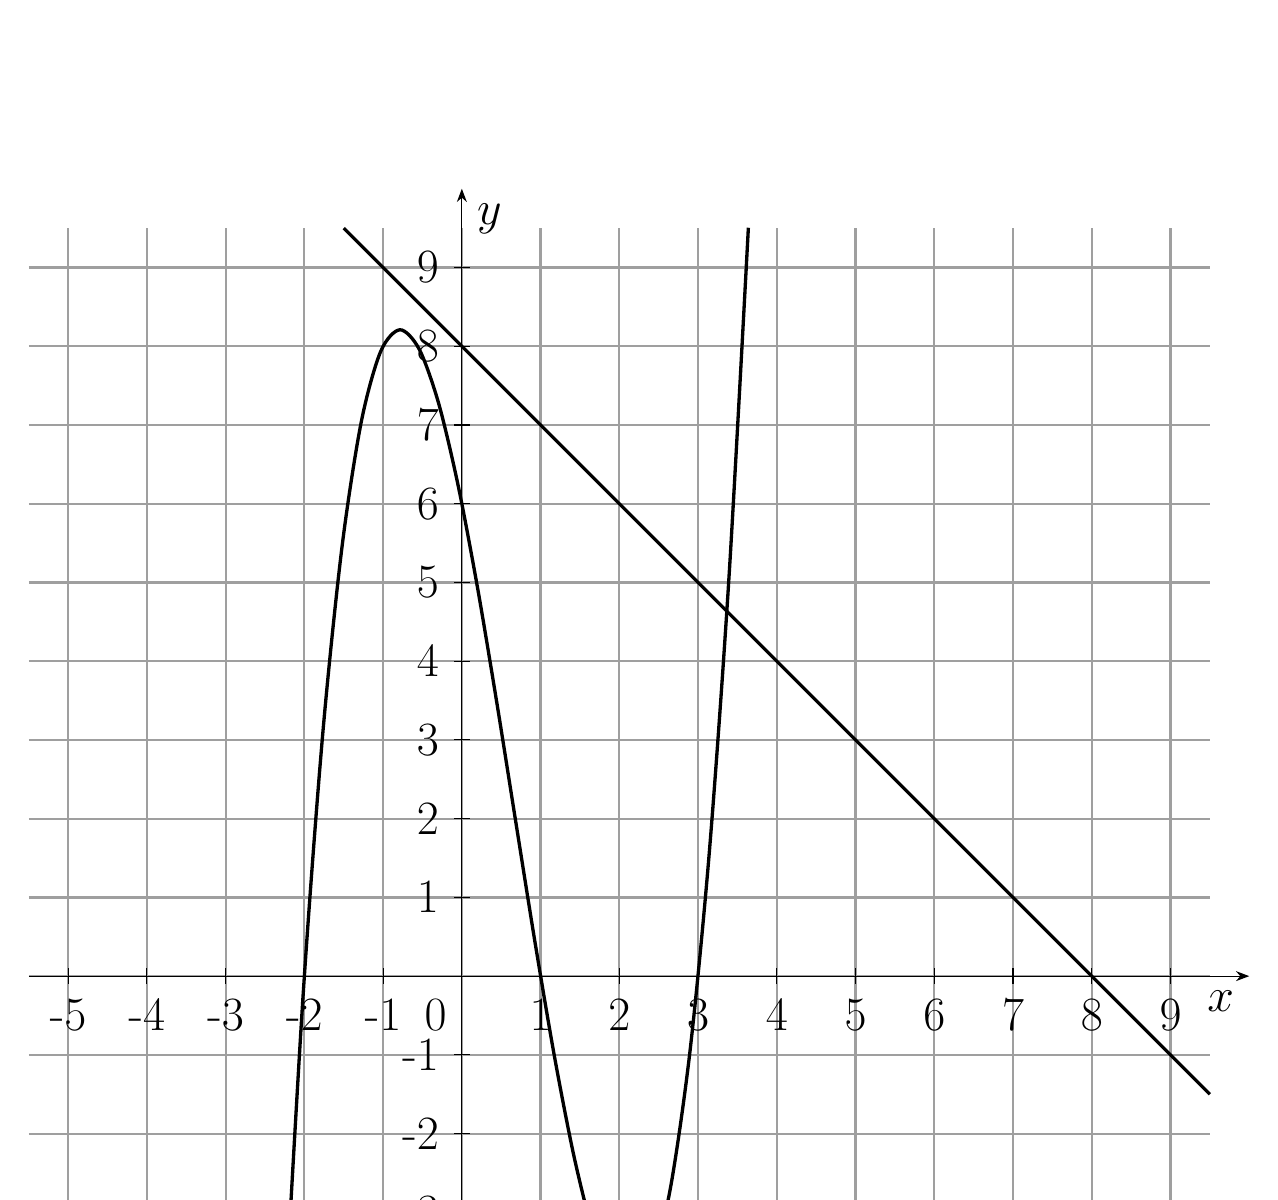
\begin{tikzpicture}[scale=1]
        % grid
        \draw[thick,gray!75] (-5.5,-4.5) grid[step=10mm] (9.5,9.5);
    
        % axis
        \draw[-Stealth] (0,-4.5) -- (0,10) node[below right] {$y$};
        \draw[-Stealth] (-5.5,0) -- (10,0) node[below left] {$x$};

        % x-axis labels
        \foreach \i in {-5,-4,...,-2,-1,1,2,...,8,9}
            \draw (\i,1mm) -- + (0,-2mm) node[below] {\i};
             % x-axis labels

        % y-axis labels
        \foreach \i in {-4,-3,...,-2,-1,1,2,...,8,9}
            \draw (1mm,\i) -- + (-2mm,0) node[left] {\i};
             % y-axis labels

   
        % plot 1
        \draw[domain=-1.5:9.5,smooth,variable=\x,black,very thick] plot ({\x},{8-\x});
   
        % plot 2
        \draw[domain=-2.262:3.639,smooth,variable=\x,black,very thick] plot ({\x},{(\x+2)*(\x-1)*(\x-3)});
   
        % label the origin
        \draw (0,1mm) -- + (0,-2mm) node[below left] {0};
    \end{tikzpicture}\\
    Find the integer value of $gff(-2)$.
    \newpage

    % Question 16
    \question You may use a calculator. The diagram below shows two touching circles, Circle L and Circle R.\\
    \begin{nscenter}
        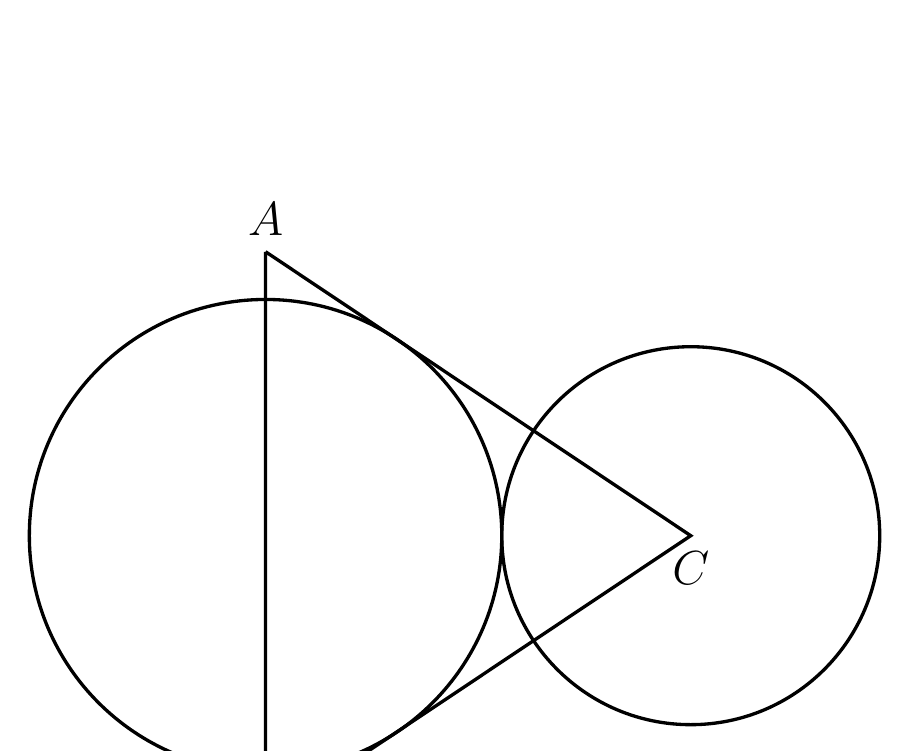
\begin{tikzpicture}[scale=0.6]
            \coordinate (O) at (0,0) {};
            \coordinate (A) at (0,6.01) {};
            \coordinate (B) at (0,-6.01) {};
            \coordinate (C) at (9,0) {};
            \draw[very thick, black] (O) circle (5){};
            \draw[very thick, black] (C) circle (4){};
            \draw[very thick, black] (A)node[anchor=south]{$A$} -- 
                  (B)node[anchor=north]{$B$} -- 
                  (C)node[anchor=north]{$C$} -- 
                  (A);
        \end{tikzpicture}
    \end{nscenter}
    Circle L has radius 5cm. Circle R has radius 4cm.\\
    $C$ is the centre of Circle R.\\
    The line $AB$ lies on the diameter of Circle L.\\
    The line $AB$ is perpendicular to a line passing through the centre of both circles.\\
    $AC$ and $BC$ are tangents to Circle L and pass through $C$.\\

    Find the area of triangle $ABC$.\\
    Give your answer to 3 significant figures.
    \newpage

    % Question 17
    \question You may use a calculator. The area of a parallelogram is $15cm^2$ correct to the nearest integer.\\
    The shortest side of the parallelogram is $4.5cm$\\ correct to 2 significant figures.\\
    The longest side of the parallelogram is $7.1cm$\\ correct to 2 significant figures.\\

    Find the largest size of the two acute angles in the parallelogram.\\
    Give your answer correct to 3 decimal places.
    
\end{questions}

\newpage
\begin{titlepage}
    \begin{center}

        \vspace*{\fill}
        \Huge \textbf{Part 3: The Exam}\\
        \vspace*{1cm}
        \vspace*{1cm}
        \large \textbf{A great filter}\\
        \vspace*{\fill}
        
    \end{center}
\end{titlepage}
\newpage
%%%%%%%%%%%%%%%%%%%%%%%%%%% Part 3

\begin{questions}

% Question 1
    \question Given that $x(a+bx)(a-bx)=25x-4x^3$, Solve for $b^{-a}$.
    \newpage

    % Question 2
    \question Freda plays the lottery.\\

    There are 49 balls to choose from.\\
    The balls are numbered 1 - 49.\\

    Freda chooses the following 6 numbers in order in which they appear:\\ 3, 4, 7, 12, 19, 28.\\
    John believes the numbers were chosen randomly.\\
    Is it possible that John is not correct? Why?
    \newpage

    % Question 3
    \question Triangle $ABC$ has the following properties:
    \begin{description}
        \item $AC=x$
        \item $BC=3x$
        \item Angle $ACB=60\degree$
    \end{description}
    Write down the perimeter of triangle $ABC$ in terms of $x$.
    \newpage

    % Question 4
    \question Find the value of $\big(\frac{1}{0.16}\big)^{1.5}$
    \newpage

    % Question 5
    \question Two students walk together along a road, starting at the same time.\\
    The speed-time graph below shows the first 9 seconds of the walk.
    
    \begin{center}
        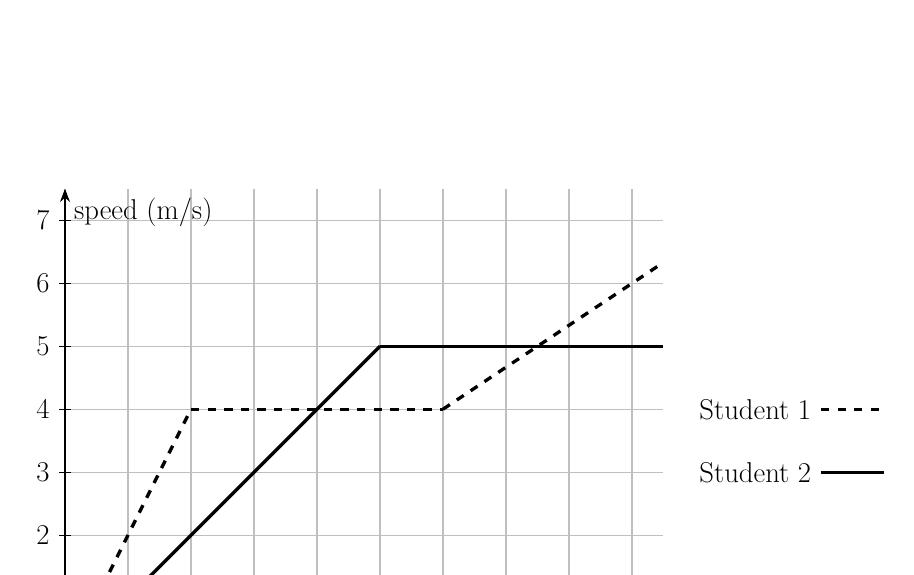
\begin{tikzpicture}[scale=0.8, every node/.style={scale=0.6}]
            % grid
            \draw[thin,gray!50] (0,0) grid[step=1] (9.5,7.5);
        
            % axis
            \draw[-Stealth] (0,-0.5) -- (0,7.5) node[below right] {speed (m/s)};
            \draw[-Stealth] (-0.5,0) -- (9.5,0) node[below right] {time (s)};
        
            % x-axis labels
            \foreach \i in {1,2,...,9}
                \draw (\i,1mm) -- + (0,-2mm) node[below] {\i};
       
            % y-axis labels
            \foreach \i in {1,2,...,7}
                \draw (1mm,\i) -- + (-2mm,0) node[left] {\i};
       
            \draw[black, very thick] (0,0) -- (5,5);
            \draw[black, very thick] (5,5) -- (9.5,5);
            
            \draw[black, very thick, dashed] (0,0) -- (2,4);
            \draw[black, very thick, dashed] (2,4) -- (6,4);
            \draw[black, very thick, dashed] (6,4) -- (9.5,6.33);

            \draw[black, very thick, dashed] (12,4) node[left] {Student 1} -- (13,4);
            \draw[black, very thick] (12,3) node[left] {Student 2} -- (13,3);
            
       
            % label the origin
            \node[anchor=north east] at (0,0) {0};
        \end{tikzpicture}
    \end{center}
    The ratio of the distance covered by Student 1 to the distance covered by Student 2 in the first 9 seconds of the walk can be written in the form $m:n$ where $m$ and $n$ are double digit integers.\\
    Find the value of $m$ and the value of $n$.
    \newpage

    % Question 6
    \question Triangle $ACD$ is shown in the diagram below.
    \begin{center}
        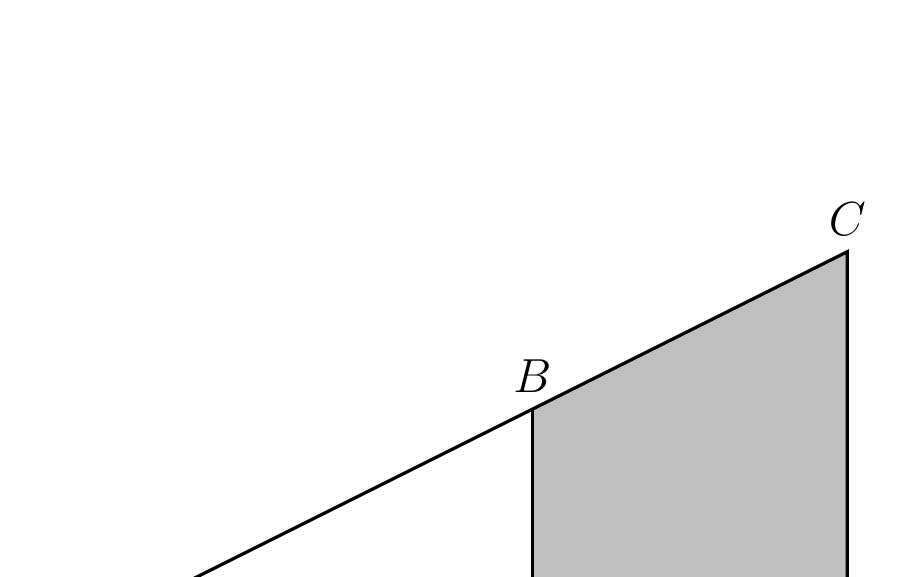
\begin{tikzpicture}
            \coordinate (A) at (0,0);
            \coordinate (B) at (6,3);
            \coordinate (C) at (10,5);
            \coordinate (D) at (10,0);
            \coordinate (E) at (6,0);
            
            \draw[draw=gray!50!white,fill=gray!50!white] 
            plot[smooth,samples=100,domain=6:10] (\x,{0}) -- 
            plot[smooth,samples=100,domain=10:6] (\x,{0.5*\x});

            \draw[very thick, black] (A) node[anchor=north] {$A$}
               -- (C) node[anchor=south] {$C$}
               -- (D) node[anchor=north] {$D$} -- (A);
            \draw[very thick, black] (B) node[anchor=south] {$B$}
               -- (E) node[anchor=north] {$E$};

            \tkzMarkRightAngle[very thick, size=0.5](C,D,E);
        \end{tikzpicture}
    \end{center}
    $AED$ is a straight line\\
    $AB=3\sqrt{5}$\\
    $AE=2BE$\\
    $3AD=5AE$\\
    $BE$ and $CD$ are parallel.\\

    Find the area of the shaded quadrilateral $BCDE$.
    \newpage

    % Question 7
    \question Evaluate: $\Big( \frac{\cos(60\degree)}{\sin(60\degree)} + \frac{10}{\sqrt{12}} \Big)^2$
    \newpage

    % Question 8
    \question You may use a calculator.\\
    $A$, $B$, $C$, and $D$ are all points on the circumference of a circle as shown in the diagram below.\\
    \begin{minipage}{0.4\textwidth}
        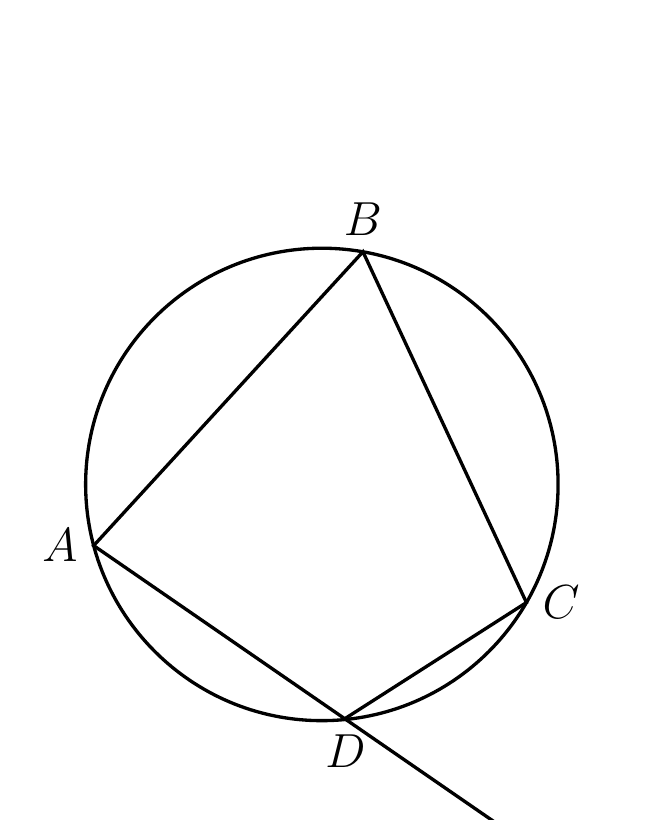
\begin{tikzpicture}[scale=3, every node/.style={scale=1}]
            \coordinate (A) at (-0.966,-0.259);
            \coordinate (B) at (0.174,0.985);
            \coordinate (C) at (0.866,-0.5);
            \coordinate (D) at (0.1,-0.99);
            \coordinate (X) at (1.14,-1.711);

            \draw[very thick, black](0,0) circle (1.0);
            \draw[very thick, black] (X) node[anchor=north] {$X$}
               -- (A) node[anchor=east] {$A$}
               -- (B) node[anchor=south] {$B$}
               -- (C) node[anchor=west] {$C$}
               -- (D) node[anchor=north] {$D$};
        \end{tikzpicture}
    \end{minipage}
    \begin{minipage}{0.4\textwidth}
    $\angle DAB = x^2-5x-8$\\
    $\angle BCD = x^2+4x-88$\\
    $\angle CDA = y^2-15y+90$\\
    $\angle ABC = 5y-6$\\
    $\angle CDX = x^2-70$\\
    Prove that $ADX$ is a straight line.
    \end{minipage}
    \newpage

    % Question 9
    \question The first five terms of an arithmetic sequence are:\\
    \begin{equation*}
        x+1 \textrm{,} \quad 2x \textrm{,} \quad \frac{2(2x+3)}{6-x} \textrm{,} \quad x^2-2 \textrm{,} \quad 5x-3
    \end{equation*}
    Show that the term $4x^2-3$ is not in the sequence.
    \newpage
    
    % Question 10
    \question A solid hemisphere piece of gold with diameter $1.2\times 10^2$cm is to be melted into identical solid cuboids.\\
    The dimensions of the cuboids are 30cm, 12cm, and 10$\pi$cm.\\
    Find the number of cuboids that can be made from the hemisphere.
    \newpage

    % Question 11
    \question Two functions are given below:
    \begin{equation*}
        f(x)=(x+p)(x+q)
    \end{equation*}
    \begin{equation*}
        g(x)=\frac{r}{x} \textrm{,} \quad x \neq 0
    \end{equation*}
    
    where $p$, $q$, and $r$ are constants.\\
    State which of the following graphs could be used to solve the equation $f(x)=g(x)$.
    
    \begin{minipage}{0.4\textwidth}
        \begin{tikzpicture}[scale=0.8, every node/.style={scale=1}]
            \draw[-Stealth] (-5,0) -- (4, 0) node[below  left] {$x$};
            \draw[-Stealth] (0,-4) -- (0,2) node[anchor=south]{$A$} node[below right] {$y$};
            
            \draw[very thick, black] plot[domain=-4.621:3.538,samples=400] (\x, {0.1*(\x*\x*\x + 2*\x*\x - 8*\x - 21)});
        \end{tikzpicture}
    \end{minipage}
    \begin{minipage}{0.4\textwidth}
        \begin{tikzpicture}[scale=0.8, every node/.style={scale=1}]
            \draw[-Stealth] (-4,0) -- (4, 0) node[below  left] {$x$};
            \draw[-Stealth] (0,-4.5) -- (0,4) node[anchor=south]{$B$} node[below right] {$y$};
            
            \draw[very thick, black] plot[domain=-2.828:2.828,samples=400] (\x, {\x*\x - 4});
        \end{tikzpicture}
    \end{minipage}\\
    \begin{minipage}{0.4\textwidth}
        \begin{tikzpicture}[scale=0.8, every node/.style={scale=1}]
            \draw[-Stealth] (-3,0) -- (6, 0) node[below  left] {$x$};
            \draw[-Stealth] (0,-2) -- (0,4) node[anchor=south]{$C$} node[below right] {$y$};
            
            \draw[very thick, black] plot[domain=-3:6,samples=400] (\x, {2-0.5*\x});
        \end{tikzpicture}
    \end{minipage}
    \begin{minipage}{0.4\textwidth}
        \begin{tikzpicture}[scale=0.8, every node/.style={scale=1}]
            \draw[-Stealth] (-2,0) -- (5, 0) node[below  left] {$x$};
            \draw[-Stealth] (0,-5) -- (0,3) node[anchor=south]{$D$} node[below right] {$y$};
            
            \draw[very thick, black] plot[domain=-1.193:4.193,samples=400] (\x, {3*\x - \x*\x});
        \end{tikzpicture}
    \end{minipage}
    \newpage

    % Question 12
    \question $A$ is inversely proportional to $B^\frac{1}{3}$ and $C$ is directly proportional to the square of $B$.\\
    When $A=0.5$, $B=64$.\\
    When $C=15$, $B=5$.\\
    Express $C$ in terms of $A$.
    \newpage

    % Question 13
    \question You may use a calculator. Mr Lucky plays two games.\\
    Playing Game A and playing Game B are independent events.\\
    The probability that Mr Lucky wins both games is $\frac{9}{25}$.\\
    The probability that Mr Lucky wins Game B is four times greater than the probability of him losing Game A.\\
    Find the probability that Mr Lucky wins only one of the two games he plays.
    \newpage

    % Question 14
    \question \phantom{1pt}
    \begin{center}
        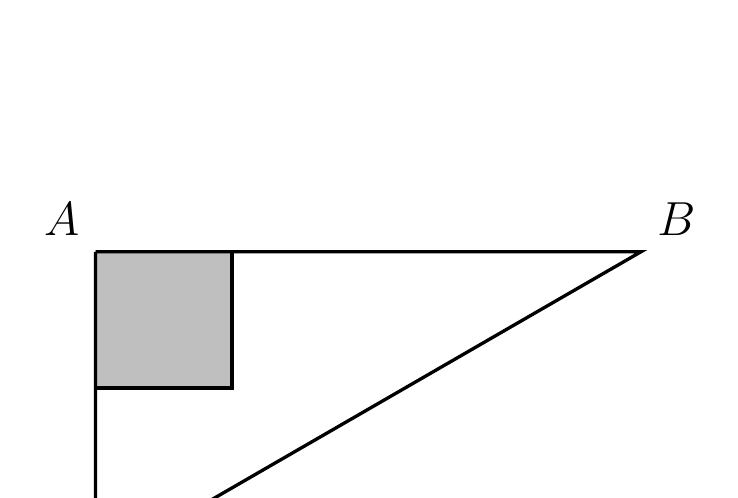
\begin{tikzpicture}[scale=4, every node/.style={scale=1}]
            \coordinate (A) at (0,0);
            \coordinate (B) at (1.732,0);
            \coordinate (C) at (0,-1);
            \coordinate (I) at (0.433,-0.433);
            \draw[draw=gray!50!white,fill=gray!50!white]  (0,0) -- (0.433,0) -- (I) -- (0,-0.433) -- (A);
            \draw[very thick, black] (A) node[anchor=south east] {$A$}
               -- (B) node[anchor=south west] {$B$}
               -- (C) node[anchor=north east] {$C$}
               -- (A);
            \draw[very thick, black] (0.433,0) -- (I) -- (0,-0.433);
        \end{tikzpicture}
    \end{center}
    Triangle $ABC$ is half of an equilateral triangle, and $\angle BAC = 90\degree$.\\
    The shaded square touches the lines $AB$ and $AC$ and the side length of the square is quarter that of $AB$.\\
    Show that the ratio of the area of the triangle to the area of the square is $8:\sqrt{3}$.
    \newpage

    % Question 15
    \question You may use a calculator. The shaded region in the diagram below is defined by three inequalities.\\
    \begin{minipage}{0.55\textwidth}
        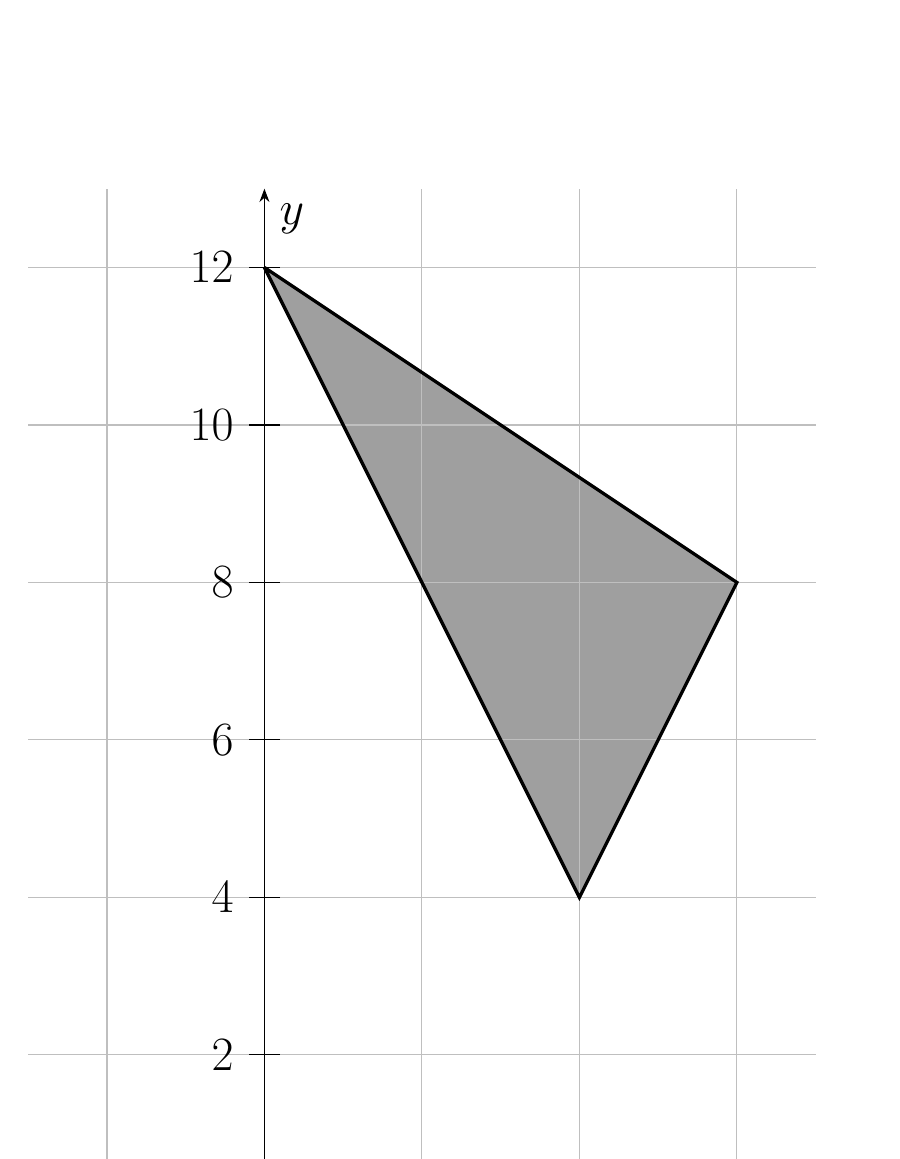
\begin{tikzpicture}[scale=2, every node/.style={scale=1}]
            % shaded region
            \draw[draw=gray!50!white,fill=gray!75!white]  (0,6) -- (3,4) -- (2,2) -- (0,6);
            % grid
            \draw[thin,gray!50] (-1.5,0) grid[step=1] (3.5,6.5);
        
            % axis
            \draw[-Stealth] (-1.5,0) -- (3.5,0) node[below right] {$x$};
            \draw[-Stealth] (0,-0.5) -- (0,6.5) node[below right] {$y$};
        
            % x-axis labels
            \foreach \i in {-0.2,0.2,0.4,0.6}
                \draw (\i*5,1mm) -- + (0,-2mm) node[below] {\i};
       
            % y-axis labels
            \foreach \i in {2,4,...,12}
                \draw (1mm,\i/2) -- + (-2mm,0) node[left] {\i};
                        
            \draw[black, very thick] (0,6) -- (3,4) -- (2,2) -- (0,6);
       
            % label the origin
            \node[anchor=north east] at (0,0) {0};
        \end{tikzpicture}
    \end{minipage}
    \begin{minipage}{0.4\textwidth}
        Find the three inequalities in the  form $ay+bx \geq c$ where $a$, $b$, and $c$ are integers.
    \end{minipage}
    \newpage

    % Question 16
    \question Two vectors are defined as follows:
    \begin{equation*}
        \overrightarrow{AC} = \begin{pmatrix}
            -2\\-1
        \end{pmatrix}
    \end{equation*}
    \begin{equation*}
        \overrightarrow{AB} = \begin{pmatrix}
            -1\\-4
        \end{pmatrix}
    \end{equation*}
    Find the value of $\cos(ACB)$ in its simplest form.
    \newpage

    % Question 17
    \question You may use a calculator. The histogram below shows information about the height (cm) of a number of plants.\\
    
    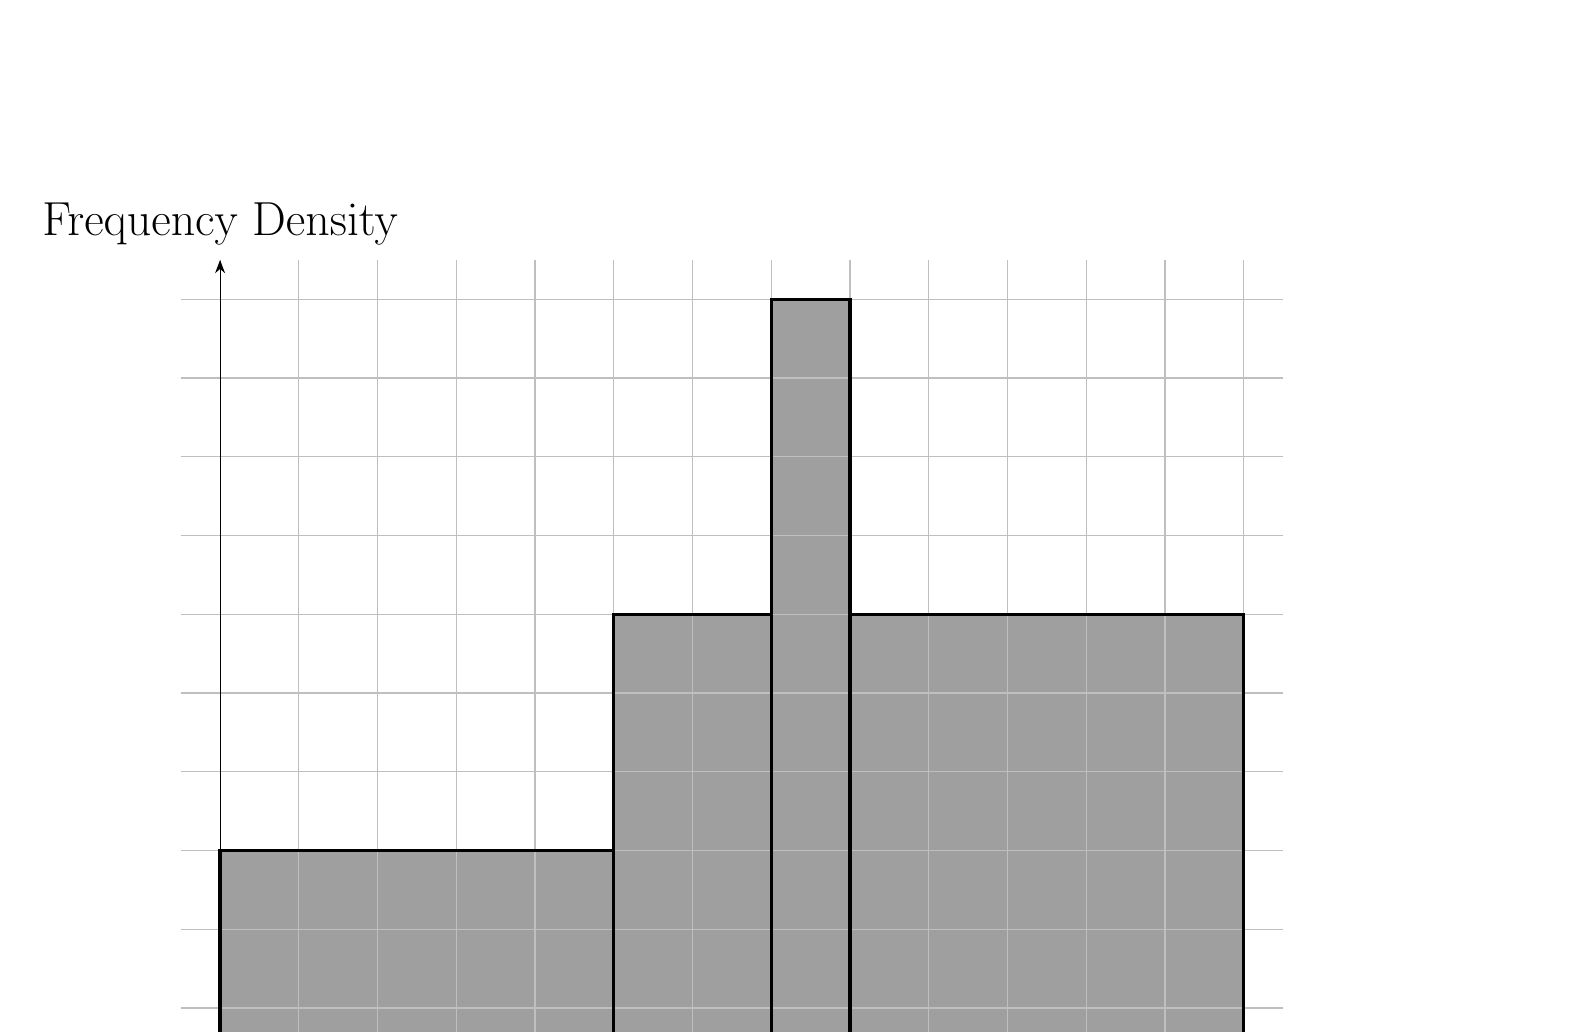
\begin{tikzpicture}[scale=1, every node/.style={scale=1}]
        % shaded region
        \draw[draw=gray!50!white,fill=gray!75!white]  (0,0) -- (0,3) -- (5,3) -- (5,6) -- (7,6) -- (7,10) -- (8,10) -- (8,6) -- (13,6) -- (13,0);
        % grid
        \draw[thin,gray!50] (-0.5,0) grid[step=1] (13.5,10.5);
    
        % axis
        \draw[-Stealth] (-0.5,0) -- (13.5,0) node[below right] {Height (cm)};
        \draw[-Stealth] (0,0) -- (0,10.5) node[above] {Frequency Density};
    
        % x-axis labels
        \foreach \i in {1,2,...,13}
            \draw (\i,1mm) -- + (0,-2mm) node[below] {\i};
                    
        \draw[black, very thick] (0,0) -- (0,3) -- (5,3);
        \draw[black, very thick] (5,0) -- (5,6) -- (7,6);
        \draw[black, very thick] (7,0) -- (7,10) -- (8,10) -- (8,6);
        \draw[black, very thick] (8,0) -- (8,6) -- (13,6) -- (13,0);
   
        % label the origin
        \node[anchor=north east] at (0,0) {0};
    \end{tikzpicture}\\
    There are 40 plants between 7 and 8cm tall.\\
    Michael takes two plants at random from the sample and doesn't replace them.\\
    He writes down his calculations for the probability and its answer as:
    \begin{equation*}
        \frac{30}{67}\times\frac{16}{89}=\frac{480}{5963}.
    \end{equation*}
    Write down the minimum height of each of the plants Michael chooses.

\end{questions}

\newpage
\begin{titlepage}
    \begin{center}

        \vspace*{\fill}
        \Huge \textbf{Part 4: The Challenge}\\
        \vspace*{1cm}
        \vspace*{1cm}
        \large \textbf{An exercise to the reader}\\
        \vspace*{\fill}
        
    \end{center}
\end{titlepage}
\newpage
%%%%%%%%%%%%%%%%%%%%%%%%%%% Part 4

\begin{questions}
% Question 1
    \question If $(ax+2)(bx+7)=15x^2+cx+14$ for all values of x, and $a+b=8$,\\ what are the two possible values for c?
    \newpage

    % Question 2
    \question The numbers $a$, $b$, and $c$ are positive integers.\\
    An apple costs £$a$, a banana costs £$b$, and a cherry costs £$c$.\\
    The costs of $b$ apples, $b$ bananas. and $a+b$ cherries is £77.\\
    What would the cost be for one apple, two bananas, and one cherry?
    \newpage

    % Question 3
    \question \phantom{1pt}\\
    \begin{minipage}{0.4\textwidth}
        In the figure, arc $SBT$ is one quarter of a circle with centre $R$ and radius 6. If the length plus width of rectangle $ABCR$ is 8, then what is the perimeter of the shaded region?
    \end{minipage}
    \begin{minipage}{0.5\textwidth}
        \begin{center}
            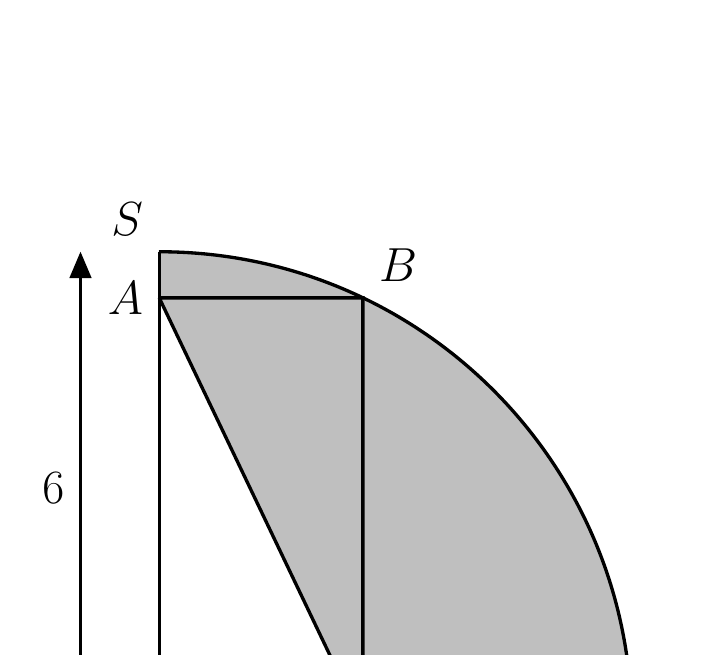
\begin{tikzpicture}
                \coordinate (R) at (0,0);
                \coordinate (A) at (0,5.414);
                \coordinate (B) at (2.586,5.414);
                \coordinate (C) at (2.586,0);
                \coordinate (T) at (6,0);
                \coordinate (S) at (0,6);
                
                \draw[draw=gray!50!white,fill=gray!50!white] (T) arc[start angle=0, end angle=90, radius=6];
                \draw[draw=gray!50!white,fill=gray!50!white] (A) -- (S) -- (T) -- (C);
                \draw[very thick, black] (S) node[anchor=south east] {$S$}
                                      -- (R) node[anchor=north east] {$R$}
                                      -- (T) node[anchor=north west] {$T$};
                \draw[very thick, black] (A) node[anchor=east] {$A$}
                                      -- (B) node[anchor=south west] {$B$}
                                      -- (C) node[anchor=north] {$C$}
                                      -- (A);
                \draw[very thick, black] (T) arc[start angle=0, end angle=90, radius=6];
                
                \draw[very thick, triangle 45-triangle 45] (-1,0) -- node[anchor= east]{6} (-1,6);
            \end{tikzpicture}
        \end{center}
    \end{minipage}
    \newpage

    % Question 4
    \question \phantom{1pt}\\
    \begin{minipage}{0.5\textwidth}
        You may use a calculator.\\
        Two congruent rectangles are shown.\\
        The are of the rectangle is 1260.\\
        The perimeter of the rectangle is 146.\\
        Find the circumference of the circle.
    \end{minipage}
    \begin{minipage}{0.3\textwidth}
        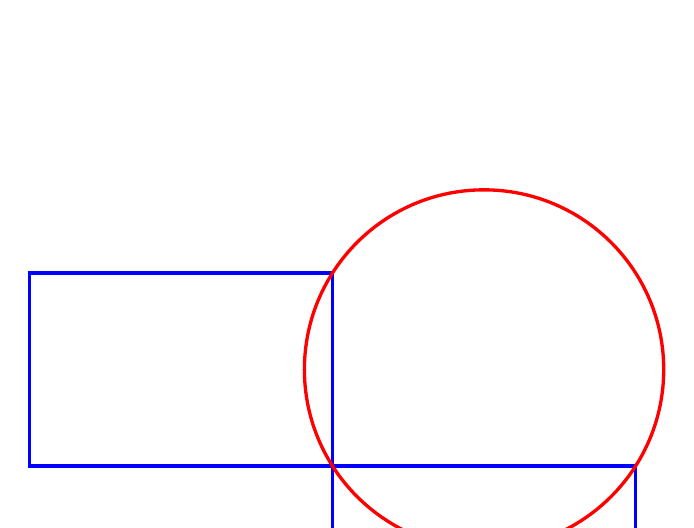
\begin{tikzpicture}[scale=0.35]
            \draw[very thick, blue] (0,0) -- (0,7) -- (-11,7) -- (-11,0) -- (11,0) -- (11,-7) -- (0,-7) -- (0,0);
            \draw[very thick, red] (5.5,3.5) circle (6.519);
        \end{tikzpicture}
    \end{minipage}
    \newpage

    % Question 5
    \question \phantom{1pt}\\
    \begin{minipage}{0.5\textwidth}
        The kite $GDBE$ is placed in the square $ACHF$.\\
        $DG=GB=EG$.\\

        Calculate the size of $x$, the angle $DBE$.
    \end{minipage} 
    \begin{minipage}{0.3\textwidth}
        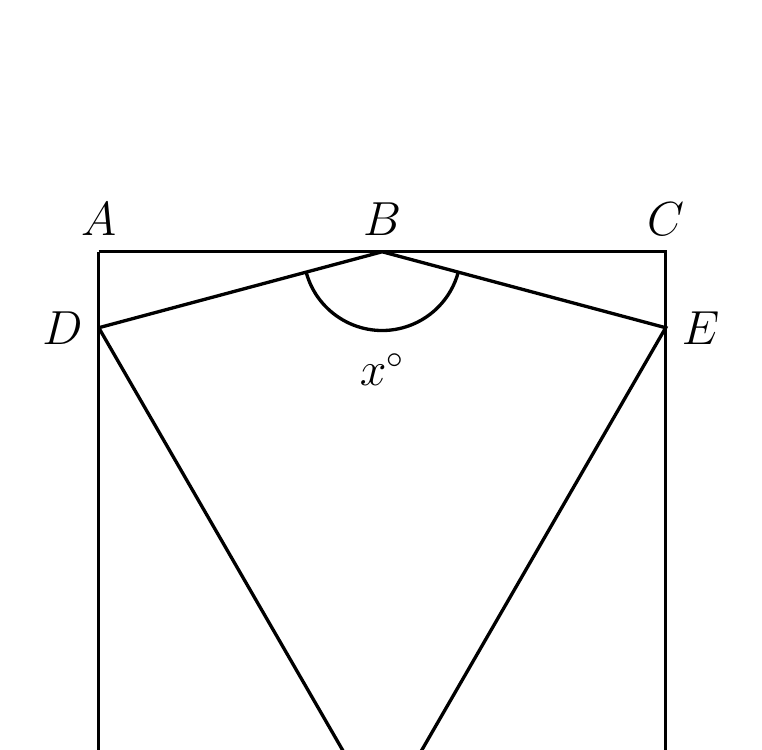
\begin{tikzpicture}[scale=0.9]
            \coordinate (A) at (0,0);
            \coordinate (B) at (4,0);
            \coordinate (C) at (8,0);
            \coordinate (D) at (0,-1.072);
            \coordinate (E) at (8,-1.072);
            \coordinate (F) at (0,-8);
            \coordinate (G) at (4,-8);
            \coordinate (H) at (8,-8);

            \draw[very thick, black] (A) node[anchor=south] {$A$}
                                  -- (C) node[anchor=south] {$C$}
                                  -- (H) node[anchor=north] {$H$}
                                  -- (F) node[anchor=north] {$F$} -- (A);
            \draw[very thick, black] (D) node[anchor=east] {$D$}
                                  -- (B) node[anchor=south] {$B$}
                                  -- (E) node[anchor=west] {$E$}
                                  -- (G) node[anchor=north] {$G$} -- (D);

            \pic [very thick, draw, -, "$x\degree$", angle eccentricity=1.5, angle radius=1cm] {angle = D--B--E};
        \end{tikzpicture}
    \end{minipage}
    \newpage

    % Question 6
    \question \phantom{1pt}\\
    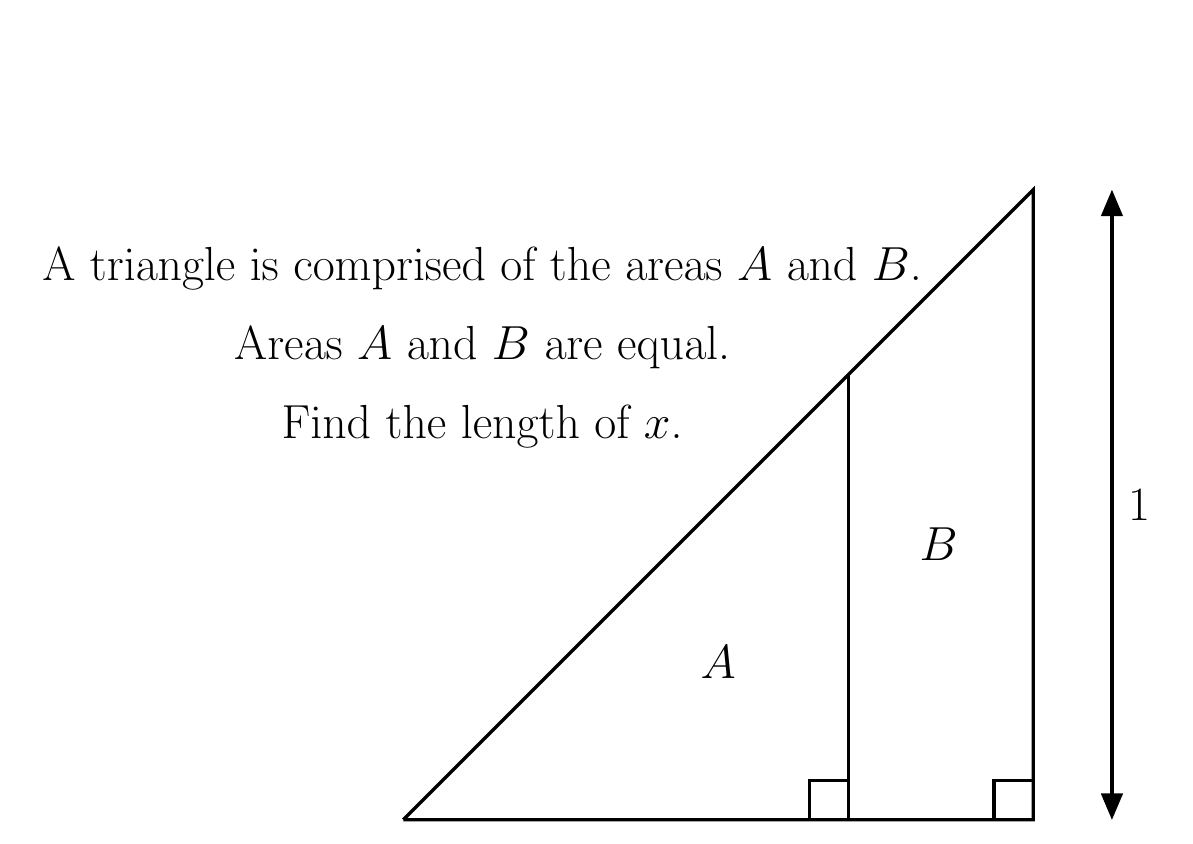
\begin{tikzpicture}[scale=1]
        \coordinate (A) at (0,0);
        \coordinate (B) at (8,0);
        \coordinate (C) at (8,8);
        \coordinate (D) at (5.657,0);
        \coordinate (E) at (5.657,5.657);
        
        \draw[very thick, black] (A) -- (B) -- (C) -- (A);
        \draw[very thick, black] (D) -- (E);
        
        \tkzMarkRightAngle[very thick, draw=black,size=.5](A,D,E);
        \tkzMarkRightAngle[very thick, draw=black,size=.5](A,B,C);

        \draw[triangle 45-triangle 45, very thick, black] (0,-0.5) -- node[anchor=north] {$x$} (5.657,-0.5);
        \draw[triangle 45-triangle 45, very thick, black] (0,-1.2) -- node[anchor=north] {$1$} (8,-1.2);
        
        \draw[triangle 45-triangle 45, very thick, black] (9,0) -- node[anchor=west] {$1$} (9,8);

        \node at (4,2) {$A$};
        \node at (6.8,3.5) {$B$};
        \node at (1,7) {A triangle is comprised of the areas $A$ and $B$.};
        \node at (1,6) {Areas $A$ and $B$ are equal.};
        \node at (1,5) {Find the length of $x$.};
    \end{tikzpicture}
    \newpage

    % Question 7
    \question \phantom{1pt}\\
    \begin{minipage}{0.5\textwidth}
        The diagram is not drawn accurately.\\$ABCD$, $EFGB$, and $ALNK$\\ are squares,\\ and $HEA$ is an equilateral triangle.\\
        Find the length of $EK$.\\
    \end{minipage}
    \hfill\vline\hfill
    \begin{minipage}{0.4\textwidth}
        Area of $EFGB$ is $36$cm$^2$.\\
        Area of $HEA$ is $27\sqrt{\frac{3}{16}}$cm$^2$.\\
        Area of $BCDLNK$ is $25$cm$^2$.\\
    \end{minipage}\\
    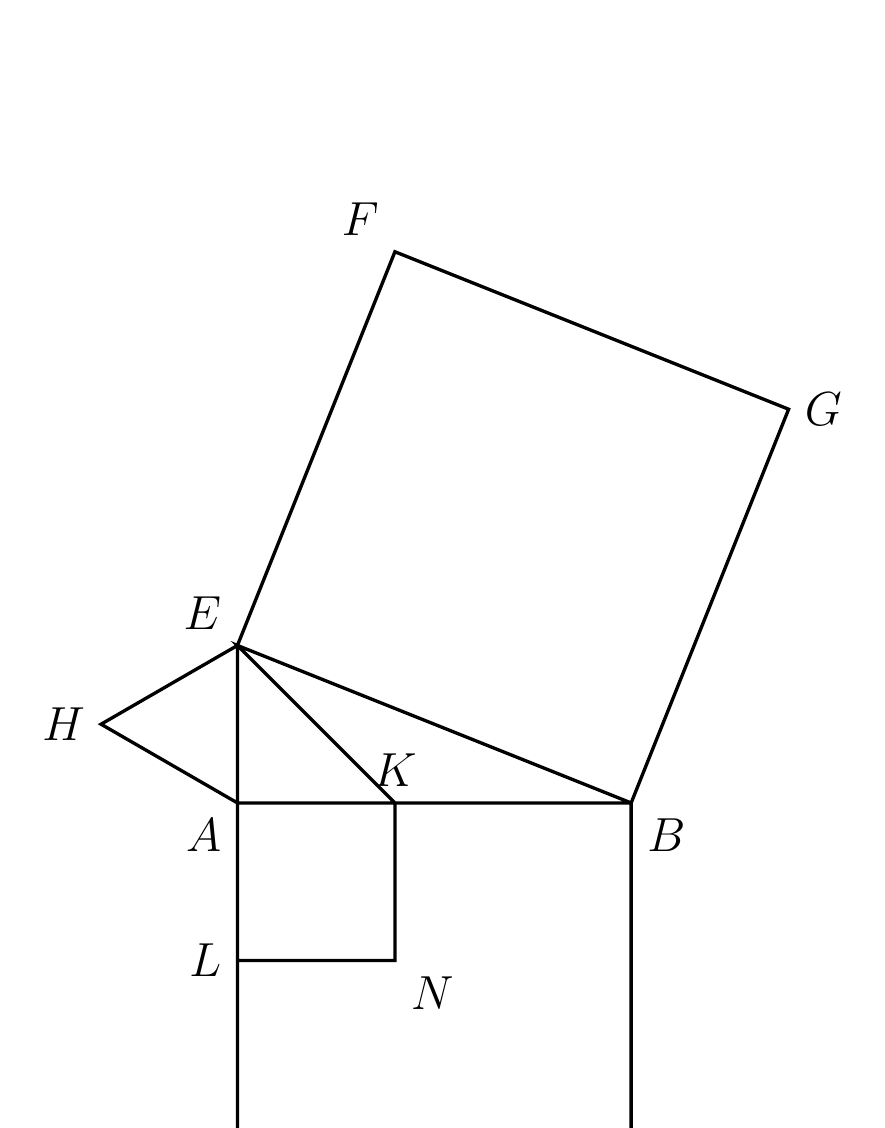
\begin{tikzpicture}
        \coordinate (A) at (0,0);
        \coordinate (B) at (5,0);
        \coordinate (C) at (5,-5);
        \coordinate (D) at (0,-5);
        \coordinate (E) at (0,2);
        \coordinate (F) at (2,7);
        \coordinate (G) at (7,5);
        \coordinate (H) at (-1.732,1);
        \coordinate (K) at (2,0);
        \coordinate (L) at (0,-2);
        \coordinate (N) at (2,-2);

        \draw[very thick, black] (A) node[anchor=north east] {$A$}
                              -- (D) node[anchor=north east] {$D$}
                              -- (C) node[anchor=north west] {$C$}
                              -- (B) node[anchor=north west] {$B$}
                              -- (A) 
                              -- (H) node[anchor=east] {$H$}
                              -- (E) node[anchor=south east] {$E$}
                              -- (F) node[anchor=south east] {$F$}
                              -- (G) node[anchor=west] {$G$}
                              -- (B) 
                              -- (E) 
                              -- (K) node[anchor=south] {$K$}
                              -- (N) node[anchor=north west] {$N$}
                              -- (L) node[anchor=east] {$L$}
                              -- (E);
    \end{tikzpicture}
    \newpage

    % Question 8
    \question Find the length of the radius of the circle.\\
    \begin{tikzpicture}[scale=0.5]
        \coordinate (A) at (17.32,10);
        \coordinate (B) at (0,0);
        \coordinate (C) at (25.32,-3.856);
        \coordinate (O) at (15.419,2.905);

        \draw[very thick, black] (A) node[anchor=south] {$A$}
                                 --  node[anchor=south] {$20$}
                                 (B) node[anchor=east] {$B$}
                                 --
                                 (C) node[anchor=north west] {$C$}
                                 --  node[anchor=west] {$16$}
                                 (A);
                              
        \draw[very thick, black] (O) circle (5.194);
        \filldraw[color=black] (O) circle [radius=.1] node[anchor= south]{$O$};
        \tkzMarkRightAngle[very thick,draw=black,size=.8](B,A,C);
        
    \end{tikzpicture}
    \newpage

    
    % Question 9
    \question Find the size of the angle at $A$.\\
    \begin{tikzpicture}[scale=0.5]
        \coordinate (A) at (17.32,10);
        \coordinate (B) at (0,0);
        \coordinate (C) at (30,-1);

        \draw[very thick, black] (A) node[anchor=south] {$A$}
                                 -- 
                                 (B) node[anchor=east] {$B$}
                                 -- node[anchor=north] {$5.8$}
                                 (C) node[anchor=north west] {$C$}
                                 --  node[anchor=south west] {$3$}
                                 (A);
                                 
        \pic [very thick, draw, -, "$28.25\degree$", angle eccentricity=1.5, angle radius=2cm] {angle = C--B--A}; 
    \end{tikzpicture}
    \newpage

    % Question 10
    \question Find the area of the circle. Each square has an area of 16.\\
    
    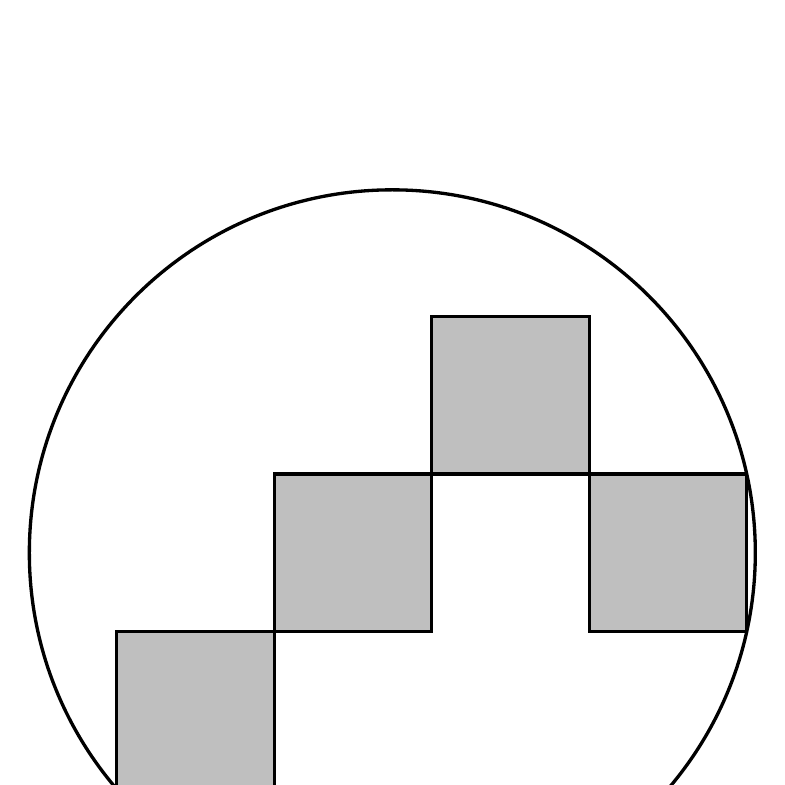
\begin{tikzpicture}[scale=0.5]
        \coordinate (O) at (7,6);
        
        \draw[very thick, draw=black,fill=gray!50!white] (0,0) -- (4,0) -- (4,8) -- (16,8) -- (16,4) -- (12,4) -- (12,12) -- (8,12) -- (8,4) -- (0,4) -- (0,0);
                              
        \draw[very thick, black] (O) circle (9.22);
        
    \end{tikzpicture}
    \newpage

    % Question 11
    \question Find the $x$ and $y$ coordinates of point $P$ in terms of radius $r$ and angle $\theta$.\\
    
    \begin{center}
        \begin{tikzpicture}   
            \coordinate (O) at (0,0);
            \coordinate (P) at (5,0);
            \coordinate (X) at (4,3);
            
            % axis
            \draw[very thick,-Stealth] (0,-7) -- (0,7) node[below right] {$y$};
            \draw[very thick,-Stealth] (-7,0) -- (7, 0) node[below  left] {$x$};
            
            % curve
            \draw[very thick, black] (0,0) circle (5cm) node[anchor=north east]{0};

            \draw[very thick, black] (0,0) -- node[anchor=south east]{$r$} (4,3) node[anchor=south west]{$P$};
            \pic [very thick,draw, -, "$\theta$", angle eccentricity=1.5, angle radius=1cm] {angle = P--O--X};
        \end{tikzpicture}
    \end{center}
    \newpage

    % Question 12
    \question \phantom{1pt}\\
    \begin{equation*}
        \text{Prove that}\phantom{1pt}\Big(x + \sqrt{x^2-1}\Big)^2=\frac{x+\sqrt{x^2-1}}{x-\sqrt{x^2-1}}\phantom{1pt}\text{.}
    \end{equation*}
    
    \newpage

    % Question 13
    \question Prove the Quadratic Formula, $x=\frac{-b\pm\sqrt{b^2-4ac}}{2a}$.
    \newpage
    
    % Question 14
    \question Show the relation between the gradients of 2 perpendicular lines.\\
    You may use the diagram below.\\
    \begin{tikzpicture}
        \coordinate (O) at (0,0);
        \coordinate (A) at (3,6);
        \coordinate (B) at (3,0);
        \coordinate (C) at (3,-1.5);
        \coordinate (D) at (-1,-2);
        \coordinate (E) at (-1,0.5);
    
        \draw[domain=-2:4,smooth,variable=\x,black,very thick] plot ({\x},{2*\x});
        \draw[domain=-4:5,smooth,variable=\x,black,very thick] plot ({\x},{-0.5*\x});
        
        \draw[very thick] (0,0) -- node[anchor=south] {$1$} (3,0);
        \draw[very thick] (3,6) -- (3,-1.5);
        
        \tkzMarkRightAngle[very thick,draw=black,size=.3](E,O,A);
        \tkzMarkRightAngle[very thick,draw=black,size=.3](O,B,A);
        \tkzMarkRightAngle[very thick,draw=black,size=.3](O,B,C);
        
    \end{tikzpicture}
    \newpage

    % Question 15
    \question Prove the Pythagorean Theorem, $a^2+b^2=c^2$.\\
    You may use the diagram below, which displays a shape with rotational symmetry of order 4.\\
    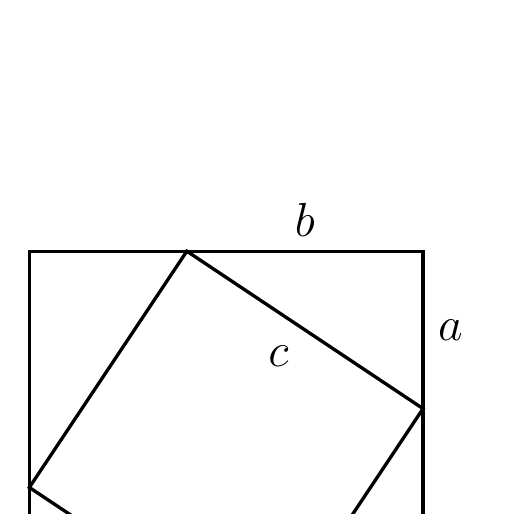
\begin{tikzpicture}
        \coordinate (A) at (0,0);
        \coordinate (B) at (0,5);
        \coordinate (C) at (5,5);
        \coordinate (D) at (5,0);
        \coordinate (E) at (3,0);
        \coordinate (F) at (5,3);
        \coordinate (G) at (2,5);
        \coordinate (H) at (0,2);

        \draw[very thick, black] (A) -- (B) -- (C) -- (D) -- (A);
        \draw[very thick, black] (E) -- (F) -- node[anchor=north east] {$c$} (G) -- (H) -- (E);

        \draw (G) -- node[anchor=south] {$b$} (C);
        \draw (C) -- node[anchor=west] {$a$} (F);
        
    \end{tikzpicture}
    \newpage

    % Question 16
    \question Prove that $\sqrt{2}$ is irrational.
    \newpage

    % Question 17
    \question Prove that the shape traced out by a quadratic, the parabola, is always symmetrical around a certain axis.\\
    Hint: You may assume that a function $f(x)$ is symmetrical around the $x=0$ axis when $f(x)=f(-x)$.
    \newpage

    % Question 18
    \question You may use a calculator.\\
    Elliott the alien is brewing themselves a cup of coffee. To brew the perfect coffee, they follow this simple formula:
    \begin{equation*}
        \xi = \frac{24\zeta -4\zeta^2 -27}{(-2\Xi+3)(\Xi-2)}
    \end{equation*}
    where $\xi$ is the perfection level of the coffee, $\zeta$ is the amount of Florp, and $\Xi$ is how much sugar is in the coffee (the units are alien, so you don't need to worry about them).\\
    Elliott measures out each of the 2 ingredients to get\\ $\zeta = 2.8$ to the nearest $0.7$,\\ and $\Xi=1.95$ to the nearest $0.05$.\\
    Calculate the maximum value for how perfect Elliott's coffee is.
    \newpage

    % Question 19
    \question You may use a calculator.\\
    \begin{minipage}{0.4\textwidth}
        Three identical cones each have a radius of 50 and a height of 120. The cones are placed such that their circular bases touch one another. Then a sphere is placed such that it rests in the space created by the three cones, as shown.
    \end{minipage}
    \hfill
    \begin{minipage}{0.4\textwidth}
        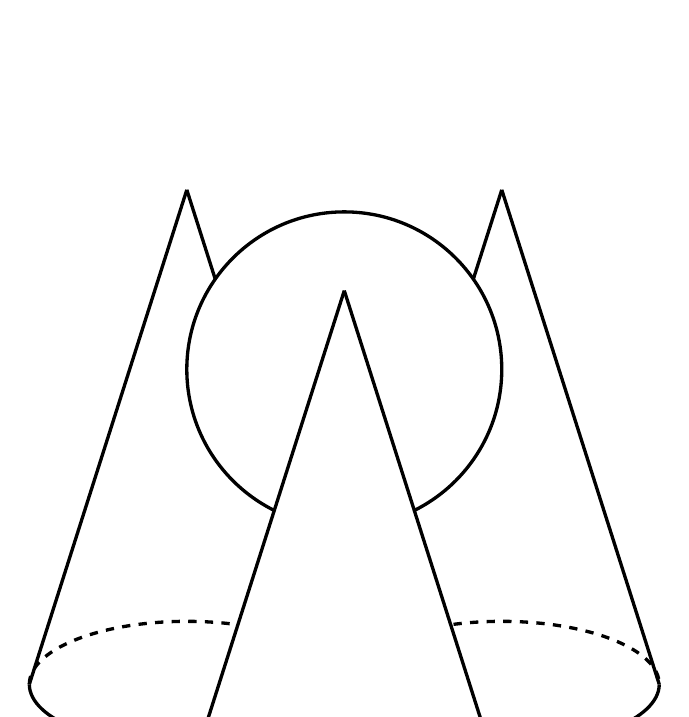
\begin{tikzpicture}[scale=0.4]
        
            \coordinate (O) at (0,0);
            \coordinate (A1) at (-5, 5.7);
            \coordinate (A2) at (5, 5.7);
            \coordinate (A3) at (0, 2.5);
            
            % Draw cone (left)
            \draw[very thick, draw=black,fill=white, dashed] (-10, -10) arc[start angle=180, end angle=0, x radius=5, y radius=2];
            \draw[very thick, draw=black,fill=white] (A1) -- ++(-5, -15.7);
            \draw[very thick, draw=black,fill=white] (A1) -- ++(5, -15.7);
            \draw[very thick, draw=black,fill=white] (-10, -10) arc[start angle=-180, end angle=0, x radius=5, y radius=2];
            
            % Draw cone (right)
            \draw[very thick, draw=black,fill=white, dashed] (0, -10) arc[start angle=180, end angle=0, x radius=5, y radius=2];
            \draw[very thick, draw=black,fill=white] (A2) -- ++(-5, -15.7);
            \draw[very thick, draw=black,fill=white] (A2) -- ++(5, -15.7);
            \draw[very thick, draw=black,fill=white] (0, -10) arc[start angle=-180, end angle=0, x radius=5, y radius=2];
            
            % Draw the sphere
            \draw[very thick, draw=black,fill=white] (O) circle (5);
            
            % Draw cone (bottom)
            \draw[draw=white,fill=white] (A3) -- ++(-5, -15.7) -- ++(10,0) -- cycle;
            \draw[very thick, draw=black,fill=white, dashed] (-5, -13.2) arc[start angle=180, end angle=0, x radius=5, y radius=2];
            \draw[very thick, draw=black,fill=white] (A3) -- ++(-5, -15.7);
            \draw[very thick, draw=black,fill=white] (A3) -- ++(5, -15.7);
            \draw[very thick, draw=black,fill=white] (-5, -13.2) arc[start angle=-180, end angle=0, x radius=5, y radius=2];
            
        \end{tikzpicture}
    \end{minipage}
        
    If the top of the sphere is the same height as the top of the cones, what is the radius of the sphere to three decimal places?
    \newpage

    % Question 20
    \question Two unit circles are joined by many equally spaced strings of length 2 to form a cylinder. The upper circle is rotated by $90\degree$ while the lower is fixed. Naturally, the two circles come closer together.\\

    What is the new distance between them?\\
    
    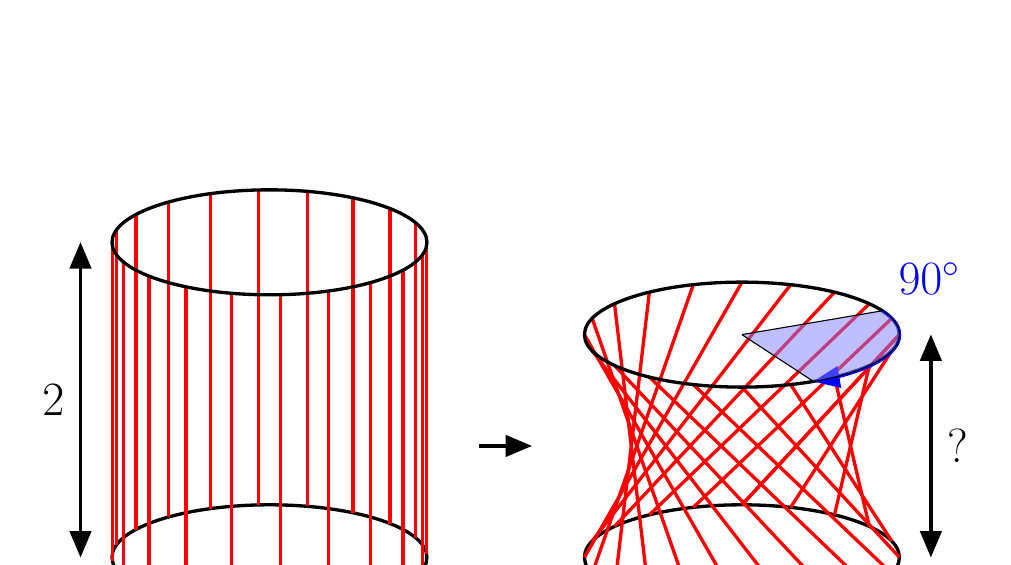
\begin{tikzpicture}[scale=2]
        % Parameters
        \def\radius{1}
        \def\height{2}
        \def\nstrings{20}
        
        % Draw the bottom circle
        \draw[very thick,black] (0, 0) arc [start angle=0, end angle=360, x radius=\radius, y radius={\radius/3}];

        % Draw the strings
        \foreach \i in {0,...,\nstrings} {
            \coordinate (top) at ({\radius*cos(360/\nstrings*\i + 22)-\radius}, {\height + 0.333*sin(360/\nstrings*\i + 22)});
            \coordinate (bottom) at ({\radius*cos(360/\nstrings*\i + 22)-\radius}, {0.333*sin(360/\nstrings*\i + 22)});
            \draw[very thick,red] (top) -- (bottom);
        }
    
        % Draw the top circle
        \draw[very thick,black] (0, \height) arc [start angle=0, end angle=360, x radius=\radius, y radius={\radius/3}];
        
        \draw[very thick, triangle 45-triangle 45] (-2.2,0) -- node[anchor=east] {2} (-2.2, \height);
        \draw[very thick, triangle 45-triangle 45] (-2*\radius,-0.5) -- node[anchor=north] {2} (0, -0.5);
        
        % Parameters
        \def\height{1.414}
        \def\offset{3}
        
        % Draw the bottom circle
        \draw[very thick,black] (\offset, 0) arc [start angle=0, end angle=360, x radius=\radius, y radius={\radius/3}];

        % Draw the strings
        \foreach \i in {0,...,\nstrings} {
            \coordinate (top) at ({\radius*cos(360/\nstrings*\i)-\radius+\offset}, {\height + 0.333*sin(360/\nstrings*\i)});
            \coordinate (bottom) at ({\radius*cos(360/\nstrings*\i + 90)-\radius+\offset}, {0.333*sin(360/\nstrings*\i + 90)});
            \draw[very thick,red] (top) -- (bottom);
        }
    
        % Draw the top circle
        \draw[very thick,black] (\offset, \height) arc [start angle=0, end angle=360, x radius=\radius, y radius={\radius/3}];

        \draw[very thick, color=blue, -triangle 45] ({\radius*cos(360/\nstrings*1.5)-\radius+\offset}, {\height + 0.333*sin(360/\nstrings*1.5)}) node[anchor=south west] {$90\degree$} arc [start angle=27, end angle=-63, x radius=\radius, y radius={\radius/3}];

        \draw[fill=blue!50!white, fill opacity=0.5] (2,\height) -- ({\radius*cos(360/\nstrings*1.5)-\radius+\offset}, {\height + 0.333*sin(360/\nstrings*1.5)}) arc [start angle=27, end angle=-63, x radius=\radius, y radius={\radius/3}] -- (2,\height);
        
        \draw[very thick, triangle 45-triangle 45] (3.2,0) -- node[anchor=west] {?} (3.2, \height);
        \draw[very thick, black, -triangle 45] (0.333,\height/2) -- (0.666,\height/2);
    \end{tikzpicture}
    \newpage

    % Question 21
    \question You may use any tool and any means, good luck.\\
     Two unit circles are joined by many equally spaced strings of length 2 to form a cylinder. The upper circle is rotated by $90\degree$ while the lower is fixed. Naturally, the two circles come closer together.\\

    What is the volume inside this 3D figure?\\
    
    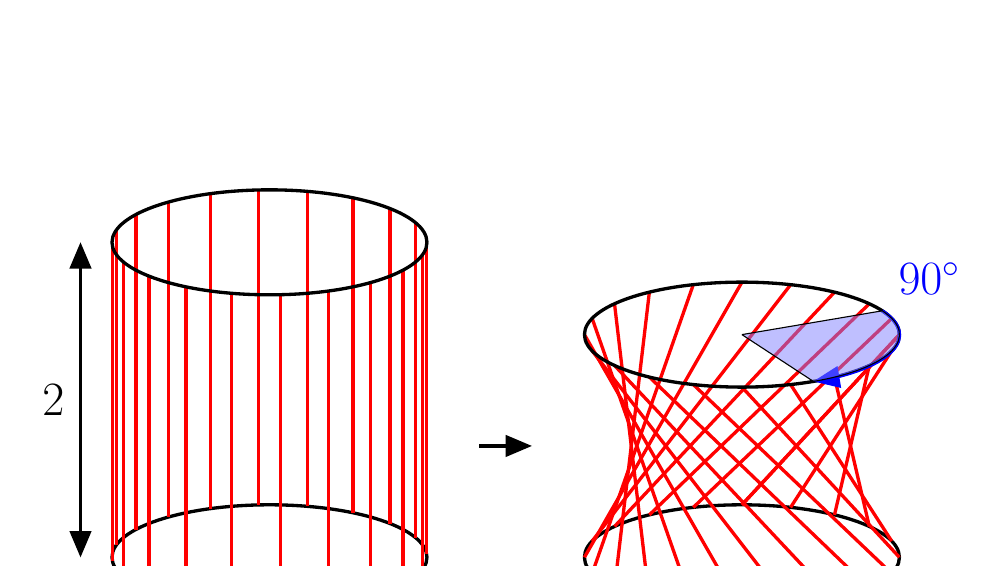
\begin{tikzpicture}[scale=2]
        % Parameters
        \def\radius{1}
        \def\height{2}
        \def\nstrings{20}
        
        % Draw the bottom circle
        \draw[very thick,black] (0, 0) arc [start angle=0, end angle=360, x radius=\radius, y radius={\radius/3}];

        % Draw the strings
        \foreach \i in {0,...,\nstrings} {
            \coordinate (top) at ({\radius*cos(360/\nstrings*\i + 22)-\radius}, {\height + 0.333*sin(360/\nstrings*\i + 22)});
            \coordinate (bottom) at ({\radius*cos(360/\nstrings*\i + 22)-\radius}, {0.333*sin(360/\nstrings*\i + 22)});
            \draw[very thick,red] (top) -- (bottom);
        }
    
        % Draw the top circle
        \draw[very thick,black] (0, \height) arc [start angle=0, end angle=360, x radius=\radius, y radius={\radius/3}];
        
        \draw[very thick, triangle 45-triangle 45] (-2.2,0) -- node[anchor=east] {2} (-2.2, \height);
        \draw[very thick, triangle 45-triangle 45] (-2*\radius,-0.5) -- node[anchor=north] {2} (0, -0.5);
        
        % Parameters
        \def\height{1.414}
        \def\offset{3}
        
        % Draw the bottom circle
        \draw[very thick,black] (\offset, 0) arc [start angle=0, end angle=360, x radius=\radius, y radius={\radius/3}];

        % Draw the strings
        \foreach \i in {0,...,\nstrings} {
            \coordinate (top) at ({\radius*cos(360/\nstrings*\i)-\radius+\offset}, {\height + 0.333*sin(360/\nstrings*\i)});
            \coordinate (bottom) at ({\radius*cos(360/\nstrings*\i + 90)-\radius+\offset}, {0.333*sin(360/\nstrings*\i + 90)});
            \draw[very thick,red] (top) -- (bottom);
        }
    
        % Draw the top circle
        \draw[very thick,black] (\offset, \height) arc [start angle=0, end angle=360, x radius=\radius, y radius={\radius/3}];

        \draw[very thick, color=blue, -triangle 45] ({\radius*cos(360/\nstrings*1.5)-\radius+\offset}, {\height + 0.333*sin(360/\nstrings*1.5)}) node[anchor=south west] {$90\degree$} arc [start angle=27, end angle=-63, x radius=\radius, y radius={\radius/3}];

        \draw[fill=blue!50!white, fill opacity=0.5] (2,\height) -- ({\radius*cos(360/\nstrings*1.5)-\radius+\offset}, {\height + 0.333*sin(360/\nstrings*1.5)}) arc [start angle=27, end angle=-63, x radius=\radius, y radius={\radius/3}] -- (2,\height);
        
        \draw[very thick, black, -triangle 45] (0.333,\height/2) -- (0.666,\height/2);
        \node (V) at (2,-0.7) {$V = $ ?};
    \end{tikzpicture}
\end{questions}

\newpage
\begin{titlepage}
    \begin{center}

        \vspace*{\fill}
        \Huge \textbf{The Sources\\(that I could find)}\\
        \vspace*{\fill}
        
    \end{center}
\end{titlepage}
\newpage
%%%%%%%%%%%%%%%%%%%%%%%%%%% Bibliography

All of Part 1 comes from the Edexcel GCSE mathematics A* paper (not for the faint of heart): \url{https://pbs.twimg.com/media/DBFJheDXYAAnLxO?format=jpg&name=4096x4096}\\

All of Part 2 comes from the GCSE 9-1 mathematics Higher Tier grade 9 "tough paper" Paper 2: \url{https://m4ths.com/uploads/3/5/2/1/35219558/new_9_to_1_grade_9_paper_2_calc.pdf}\\

All of Part 3 comes from the GCSE 9-1 mathematics Higher Tier grade 9 "tough paper" Paper 1: \url{https://m4ths.com/uploads/3/5/2/1/35219558/357.pdf}\\

Part 4 question 1 comes from Part 3 question 15 of the SAT practice test #1: \url{https://cdn2.hubspot.net/hubfs/360031/PrepScholar-sat-practice-test-1.pdf}\\ 

Part 4 question 2 comes from an early round of the norwegian mathematical olympiad, detailed in a Mind your decisions video: \url{https://www.youtube.com/watch?v=yBW-saaH-PQ}\\

Part 4 question 3 comes from the official SAT study guide, detailed in a Mind your decisions video: \url{https://www.youtube.com/watch?v=CyOhrcZsXmg&t=19s}\\

Part 4 question 4 does not have a known source, please let me know if you know the origins of this problem.\\

Part 4 question 5 comes from the NZQA Level 1 mathematics and statistics Exam 2017, detailed in a Mind your decisions video: \url{https://www.youtube.com/watch?v=z3zjyCZFzDo}\\

Part 4 question 7 is a modified version of a problem I can't find the source of, but the original problem was not solvable (I added the equilateral triangle and its area)\\

Part 4 question 8 comes from the CCEA A-level Maths past papers June 2017 Module C2:AS Core Mathematics 2 AMC21: \url{https://revisionmaths.com/level-maths/level-maths-past-papers/ccea-level-maths-past-papers}\\

Part 4 question 9 was a question I argued with my teacher about when I was still doing my GCSEs, if you have seen this problem before, please tell me its origin.\\

Part 4 question 10 comes from an Andy maths video: \url{https://www.youtube.com/watch?v=R0K__9RcF78}\\

Part 4 question 19, question 20, and question 21 all come from Brilliant daily problems, which have been discontinued\\

All questions not mentioned in the list above come from my strange mind.\\

\end{document}